The hadronic signature in ``mono-$Z$'' events ($Z \to q\bar{q}$ events in association with 
large missing transverse momentum) 
is considered to be complement to the mono-$Z$ leptonic signature described previously.
Potentially the hadronic signature will allow us to probe, compared to the leptonic one, 
the model parameters involving higher-mass CP-even Higgs boson 
due to increased branching fraction for the $Z$ decay,
while it generally suffers more from larger background in the low mass region.
The mono-$Z$ hadronic signature is therefore expected to provide additional sensitivity to the model, possibly 
extending the reach to a higher mass region.

\paragraph{Technical setup :}
Simulation of mono-$Z$ hadronic events is performed using a setup similar to that used for the leptonic events. 
The Madgraph5\_aMC@NLO version 2.4.3, interfaced with Pythia version 8.212 for parton showering 
and the LO NNPDF3.0 with $\alpha_{S}(M_{Z}) = 0.130$ for PDF in the matrix element calculations, 
is used for the event generation. 
Only gluon-gluon initial states are considered for the production of mono-$Z$ events. 
In contrast to the leptonic case, the $Z$-boson is explicitly required in the intermediate state ({\tt g g > xd xd$\sim$ z}) 
to ensure that non-$Z$ hadronic events are suppressed in the produced sample. 
The MadSpin is used for the $Z$ decay to maintain a proper spin correlation between the $Z$ decay quarks.
 
\paragraph{Event selection :} 
For mono-$Z (\to q\bar{q})$ events intermediated by the exchange of a high-mass CP-even $H$ boson, 
the $Z$-boson will be produced with 
a large transverse momentum and the hadronic decay products of such $Z$-boson could be merged into a single jet. 
Such ``boosted'' event topology is investigated by exploiting the reconstruction technique with 
a large-radius jet (denoted by $J$), 
in addition to more conventional ``resolved'' event topology where the $Z$ decay products are reconstructed 
as two separate
small-radius jets (denoted by $j$). The jet reconstruction and the following analysis are all performed at particle level
after showering and hadronization implemented in Pythia 8.212 described above.

Two consecutive stages of event selection are considered for the boosted and resolved event topologies:
\begin{itemize}
\item Inclusive: minimal kinematic requirements are applied to a pair of small-radius jets (a single large-radius jet) 
for the resolved (boosted) event topology. 
The resolved and boosted selection cuts are applied separately, i.e, not sequentially.
\item Final selection: cuts are applied to the variables used to define the signal selections. The invariant mass of the pair 
of small-radius jets or the single large-radius jet is required to be within a window around the $Z$ mass. 
In addition, selection is applied to the azimuthal angular difference between the $\chi\overline{\chi}$ and 
the hadronic $Z$-boson system, $\Delta\Phi(jj {\,\text{or}\,} J, \MET)$, and the magnitude of $\MET$.
These final selection cuts are applied sequentially to mimic a realistic analysis; in this study the boosted selection
cuts are applied first and then the resolved selection cuts are applied to those events that fail the boosted ones.
\end{itemize}

The event selection criteria used in the following analysis are listed in Table~\ref{tab:monozqq_selection}.

\begin{table}
\centering
\caption{Event selections used in the analysis for the mono-$Z$ hadronic signature with $Z \to q\bar{q}$ decays.
        The requirements are inspired from those used in a typical experimental analysis. 
        The $j$ ($J$) stands for the small-radius (large-radius) jet in the resolved (boosted) analysis.}
\begin{tabular}{c|c|r}
Selection stage & Quantity & Requirement \\\hline

\multirow{ 4}{*}{Inclusive resolved and boosted selections}  & Jet radius & $=0.4$ (1.0)\\
                                          & Jet $\left|\eta\right|$  & $<2.5$ (2.0)\\
                                          & Jet \pt                       & $>25$ GeV (200)\\
                                          & Number of jets         & $\geq2$ (1)\\\hline
\multirow{ 3}{*}{Final resolved and boosted selections}   & $|m_{jj {\,\text{or}\,} J} - m_Z|$             & $<15$ GeV\\
                                                    & $\Delta\Phi(jj {\,\text{or}\,} J, \MET)$    & $>2$\\
                                                    &  $\MET$                             & $>100$ (250) GeV\\
\end{tabular}
\label{tab:monozqq_selection}
\end{table}


\paragraph{Results :} 

\begin{figure}
\centering
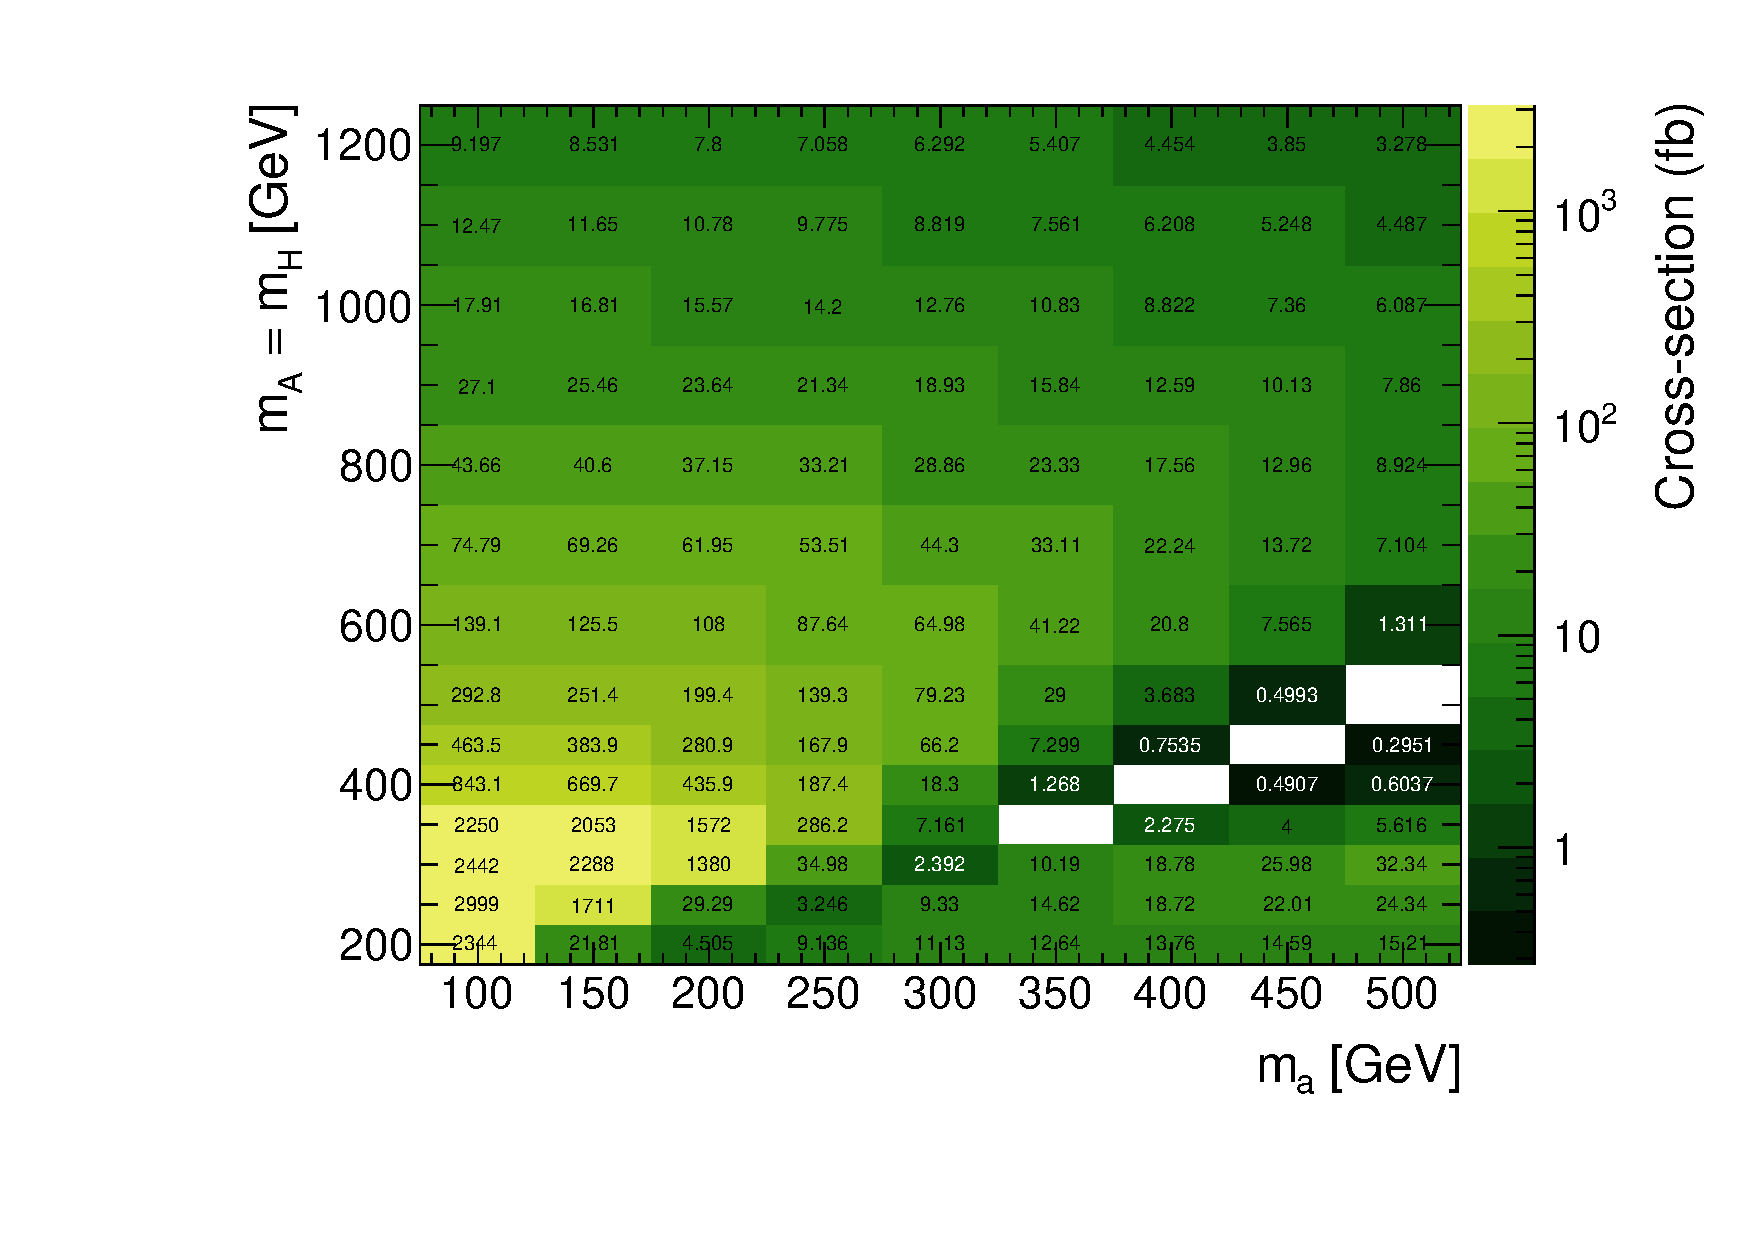
\includegraphics[width=0.45\textwidth]{texinputs/04_grid/figures/monoz/hadronic/grid_mA_ma_xsec.pdf}
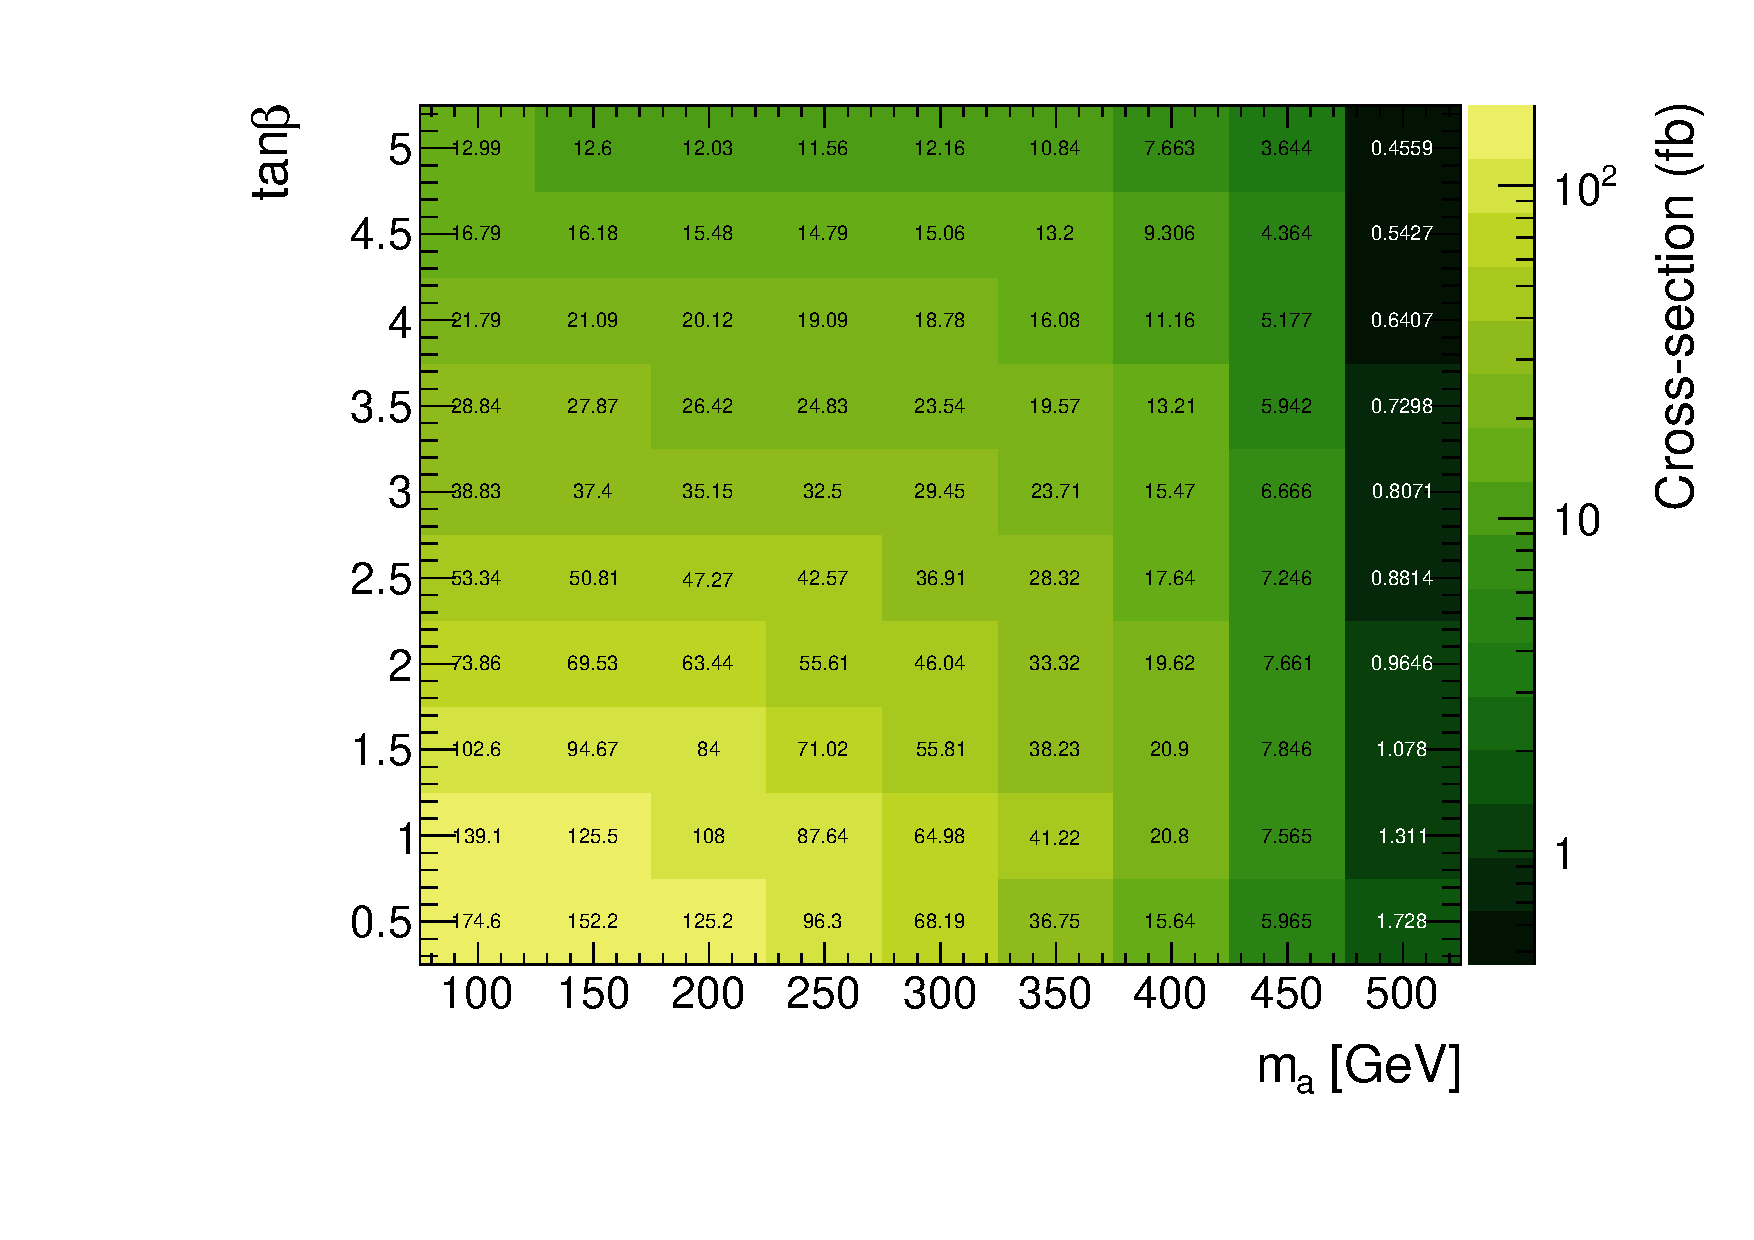
\includegraphics[width=0.45\textwidth]{texinputs/04_grid/figures/monoz/hadronic/grid_tanb_ma_xsec.pdf}
\caption{Inclusive cross-sections for the mono-$Z$ hadronic events 
$pp \rightarrow Z(\to q\bar{q})\chi\overline{\chi}$ in the \ma vs \mA (left) and \ma vs $\tan\beta$ (right) grids.
The $Z \to q\bar{q}$ branching fraction is not included in the cross-section.}
\label{fig:monozhad_inc_xsec_grid}
\end{figure}

Figure~\ref{fig:monozhad_inc_xsec_grid} shows the production cross-section for mono-$Z$ events 
in the $M_a$ ($M_A$) range between 100 and 500~GeV (200 and 1200~GeV). Shown on the left (right) is 
the cross-section in the \ma vs \mA (\ma vs $\tan\beta$) grid. Note that the $Z \to q\bar{q}$ branching fraction 
is not included in the cross-section. The production cross-section 
tends to vanish in the region where the $M_a$ gets close to $M_A$, as shown by the empty points in the grid.


\begin{figure}
\centering
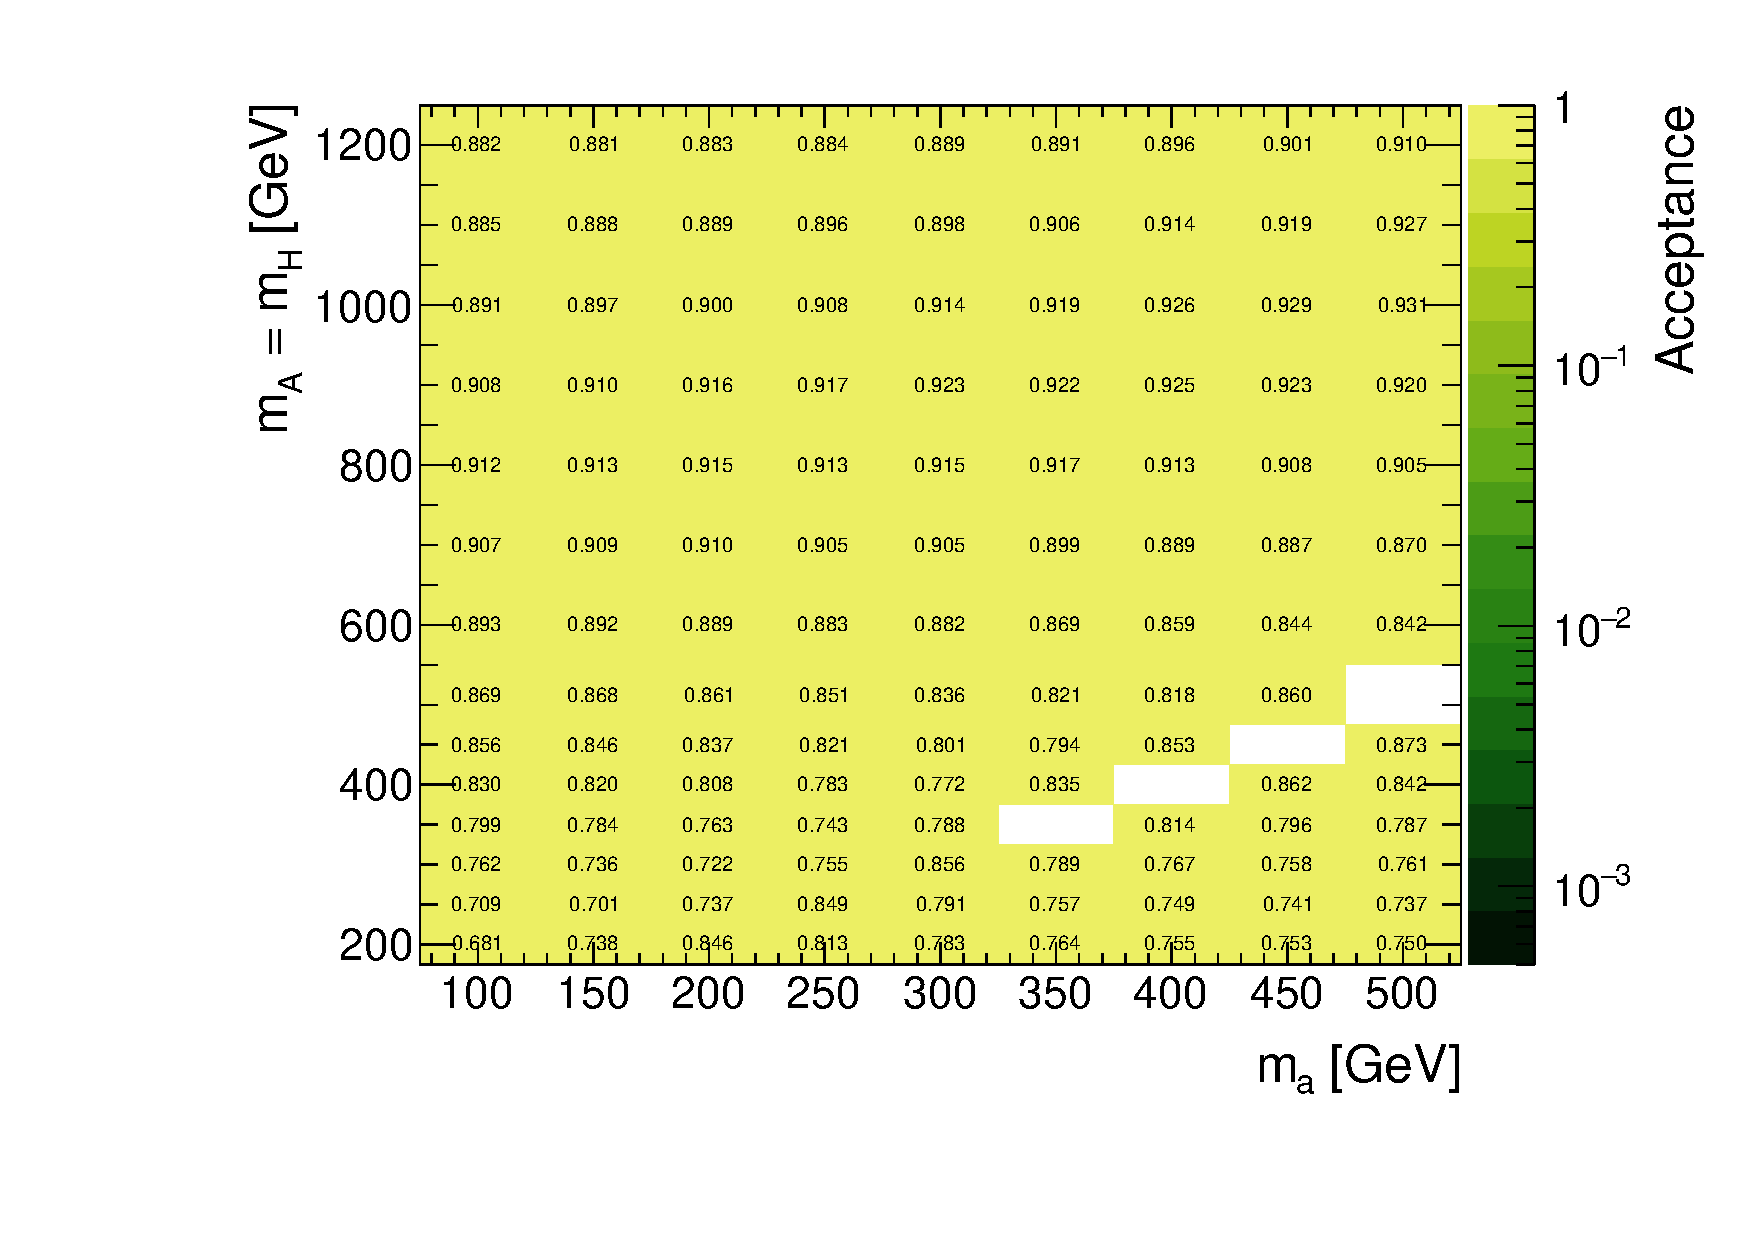
\includegraphics[width=0.45\textwidth]{texinputs/04_grid/figures/monoz/hadronic/grid_mA_ma_incl_resl_acc.pdf}
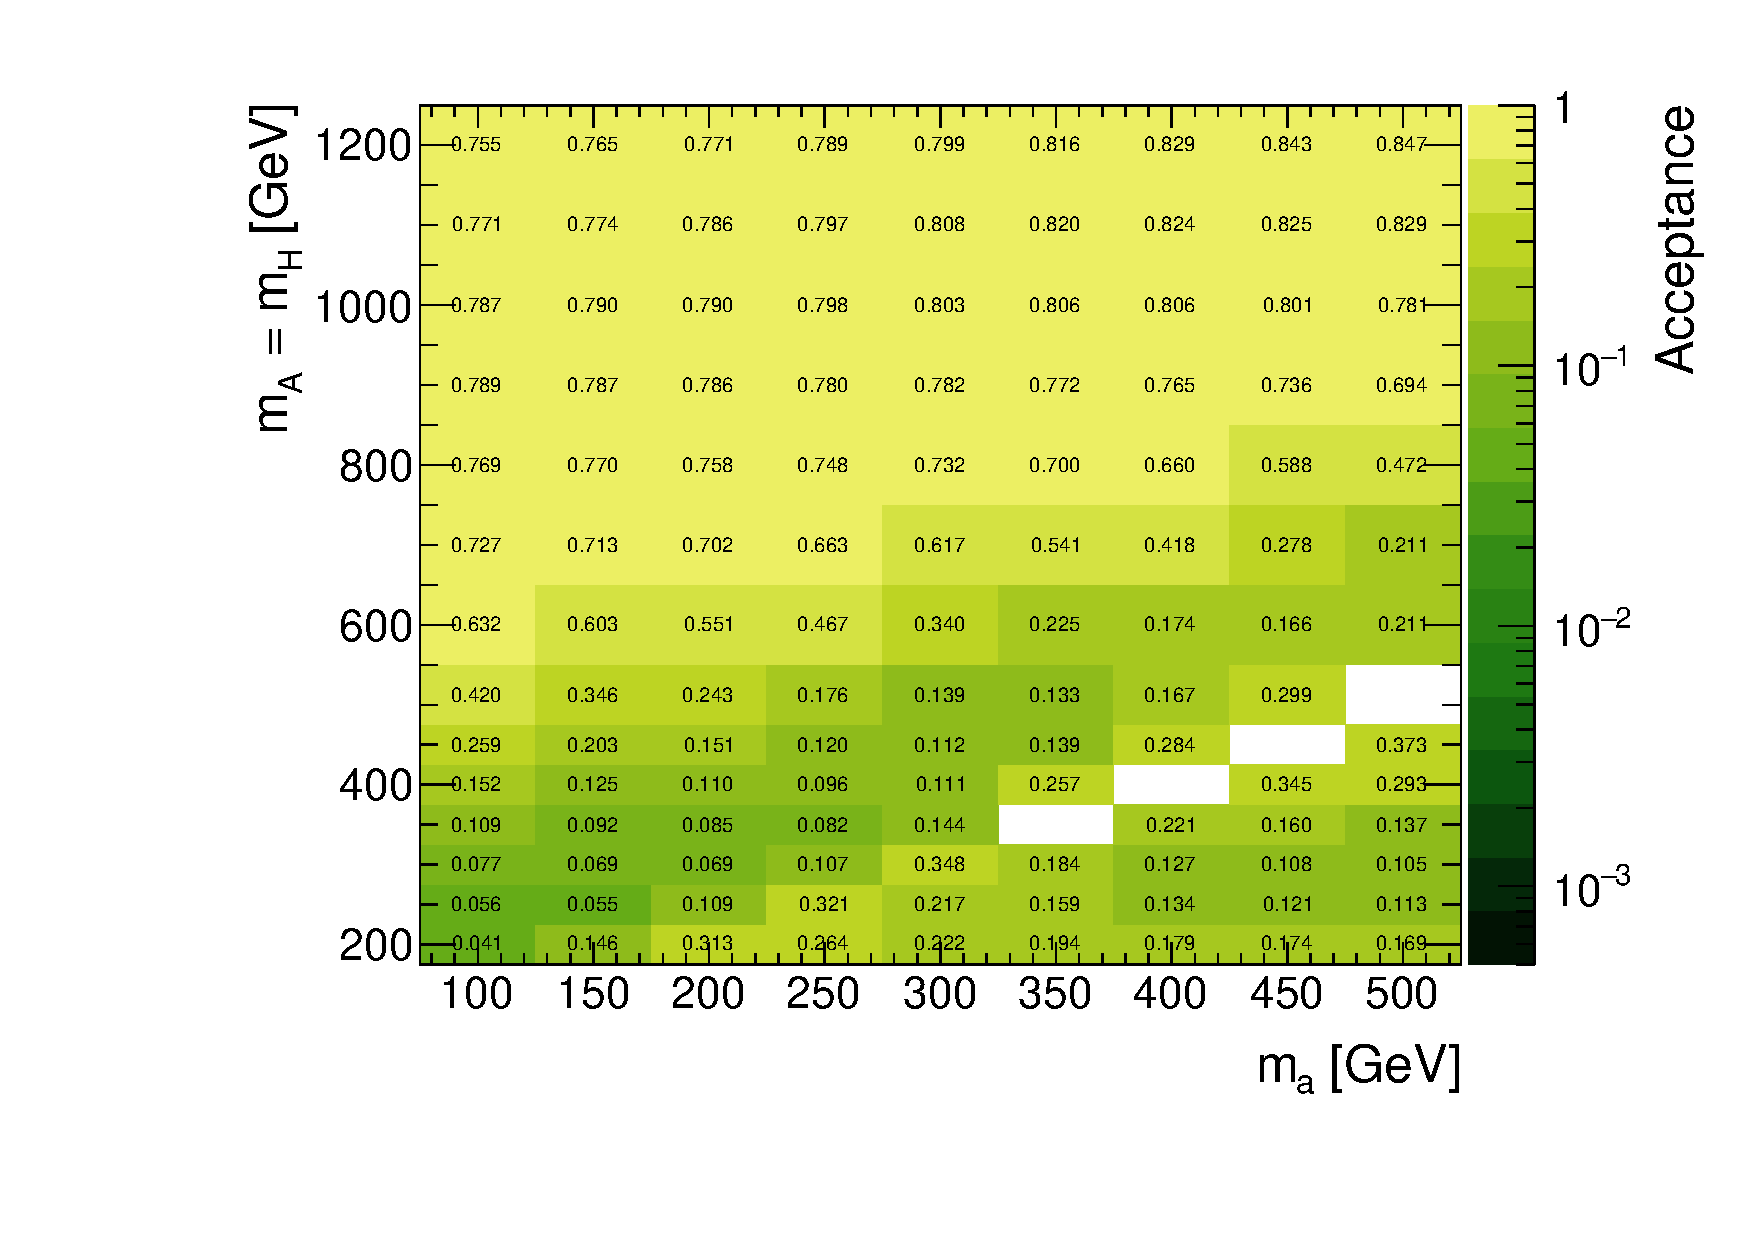
\includegraphics[width=0.45\textwidth]{texinputs/04_grid/figures/monoz/hadronic/grid_mA_ma_incl_merged_acc.pdf}
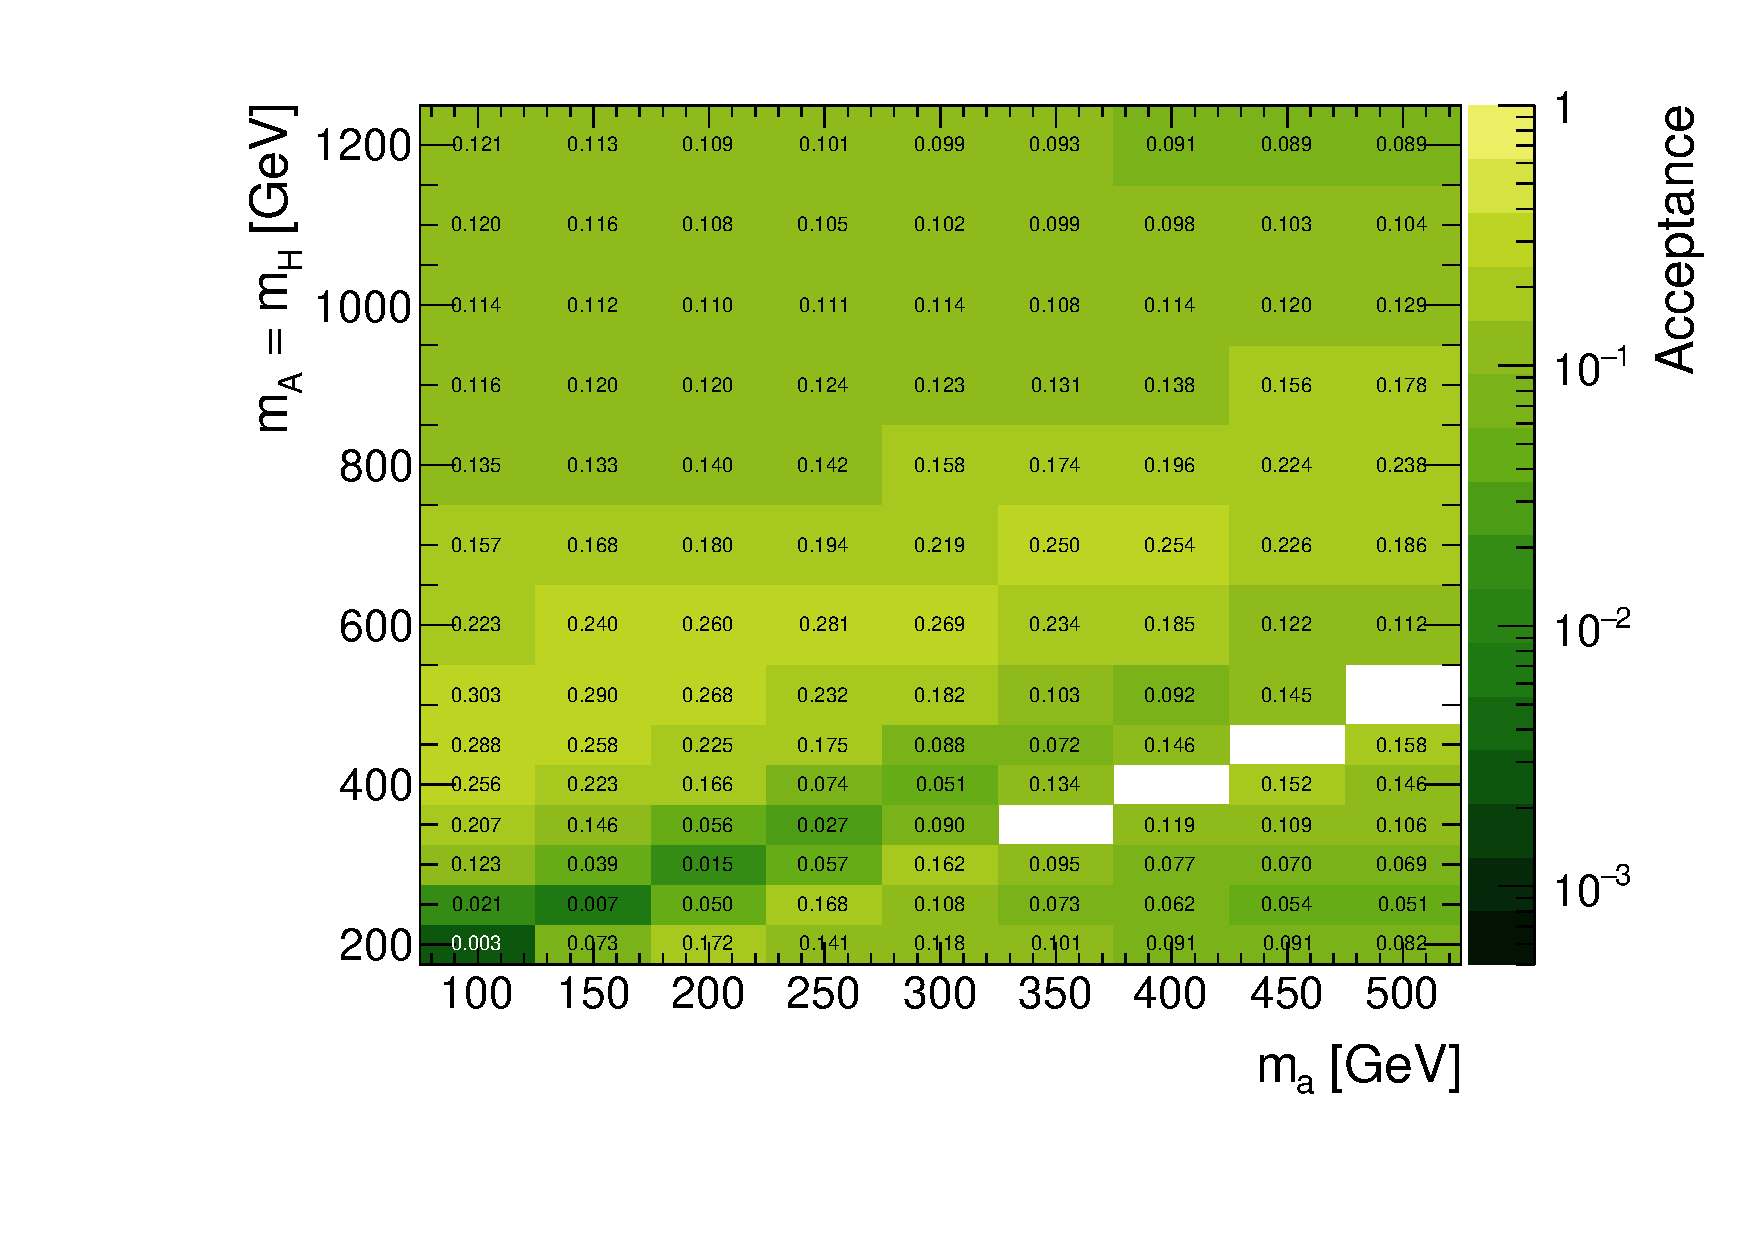
\includegraphics[width=0.45\textwidth]{texinputs/04_grid/figures/monoz/hadronic/grid_mA_ma_resl_acc.pdf}
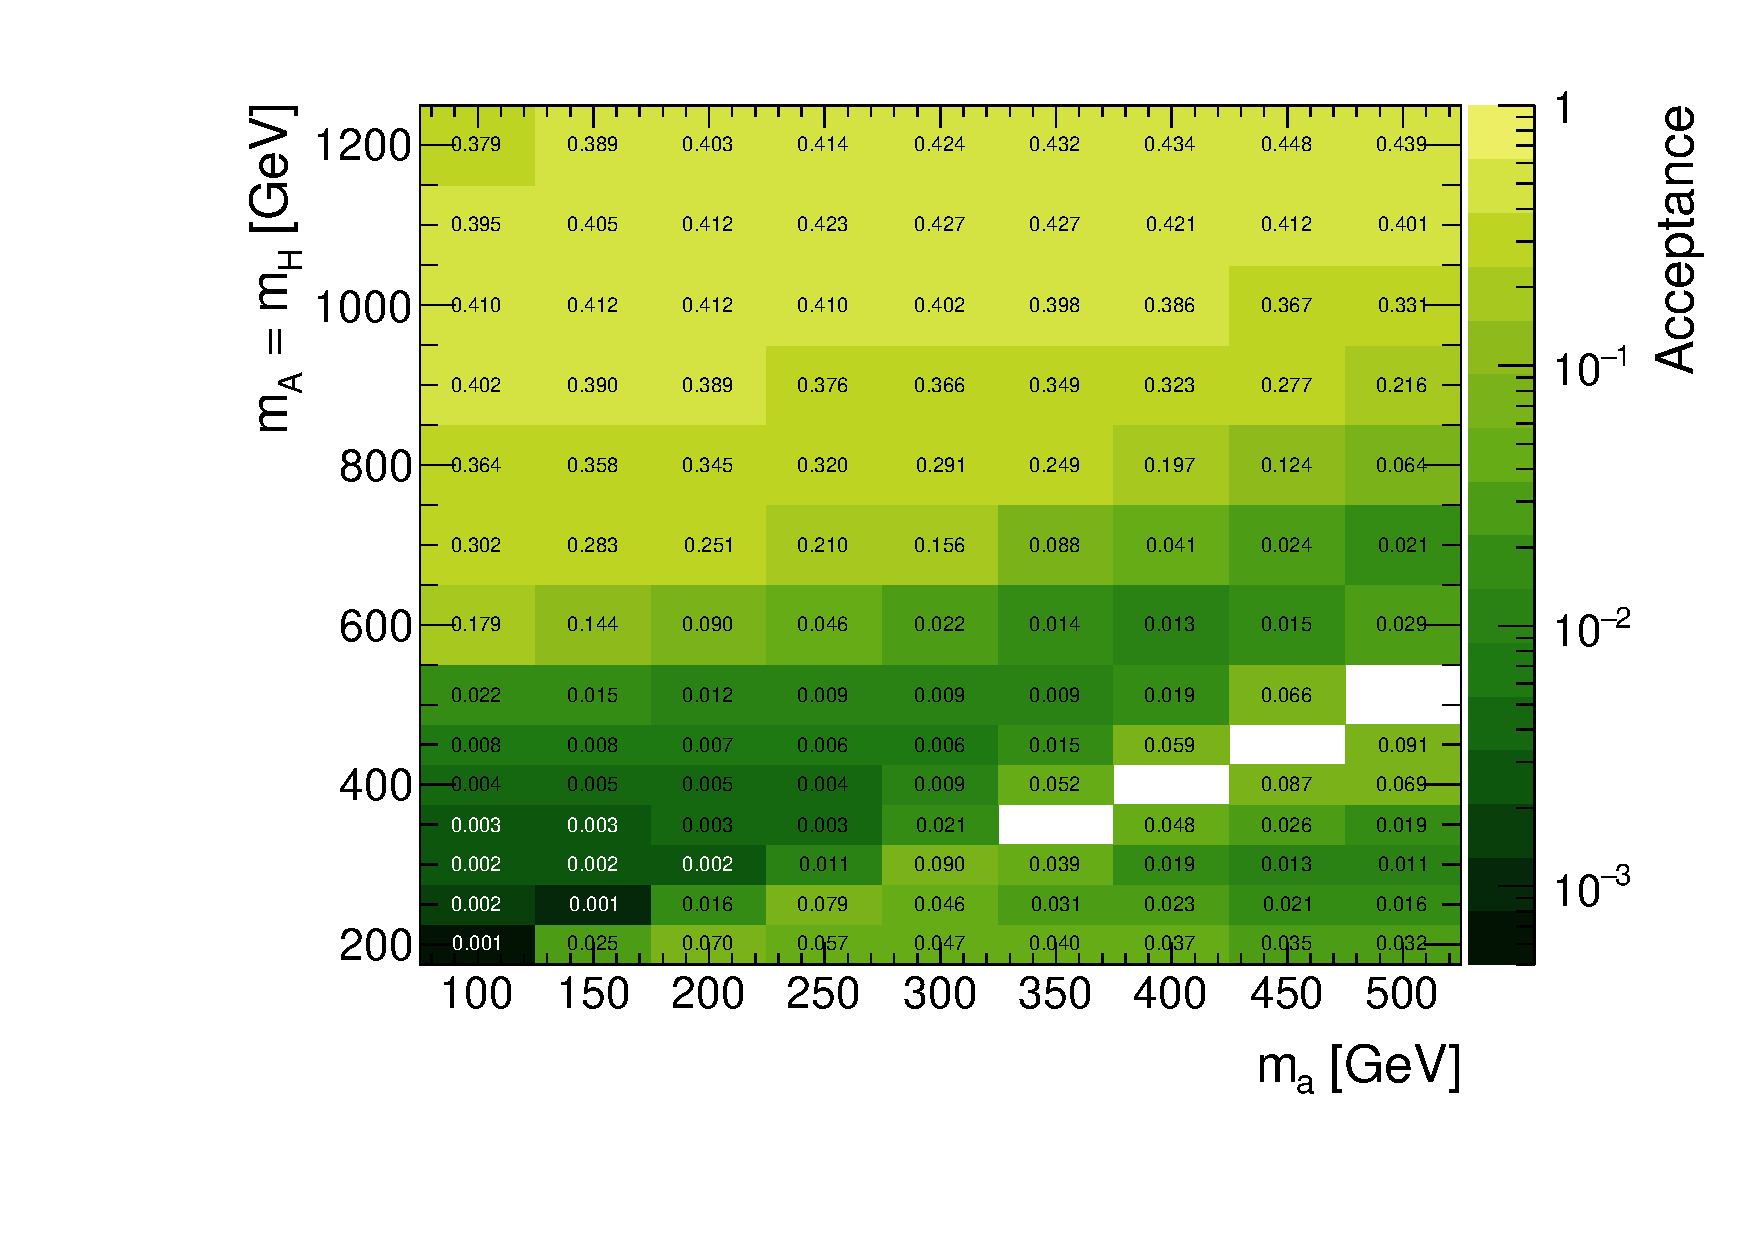
\includegraphics[width=0.45\textwidth]{texinputs/04_grid/figures/monoz/hadronic/grid_mA_ma_merged_acc.pdf}
\caption{Acceptance for the inclusive (top) and final (bottom) selections for the mono-$Z$ hadronic events 
$pp \rightarrow Z(\to q\bar{q})\chi\overline{\chi}$ in the \ma vs \mA grid. Shown on the left (right) is the acceptance for
the resolved (boosted) analysis selections.}
\label{fig:monozhad_acc_ma-mA_grid}
\end{figure}

The signal acceptance for the four sets of event selections given in Table~\ref{tab:monozqq_selection} is 
summarized in Fig.~\ref{fig:monozhad_acc_ma-mA_grid} in the \ma vs \mA grid. Note again that the resolved and boosted 
selection criteria are applied separately for the inclusive case, while for the final selections the boosted criteria are 
applied first and then the resolved ones to those failing the boosted criteria. 
For the inclusive case, the mass dependence on the acceptance is weak for the resolved criteria 
while it is rather significant for the boosted criteria 
as the $Z$-boson is less boosted with decreasing \mA and hence less likely that the $Z$-decay products are merged 
into a single jet. The final boosted selections have acceptance larger than $\sim20$\% (40\%) at 
$\mA>800$ (1000)~GeV and $\ma<400$~GeV. The final resolved selections can recover 10-20\% of signal 
events which fail the boosted criteria in the same mass regions. At $\mA<600$~GeV the signal acceptance 
is dominated by the resolved selection criteria.


\begin{figure}
\centering
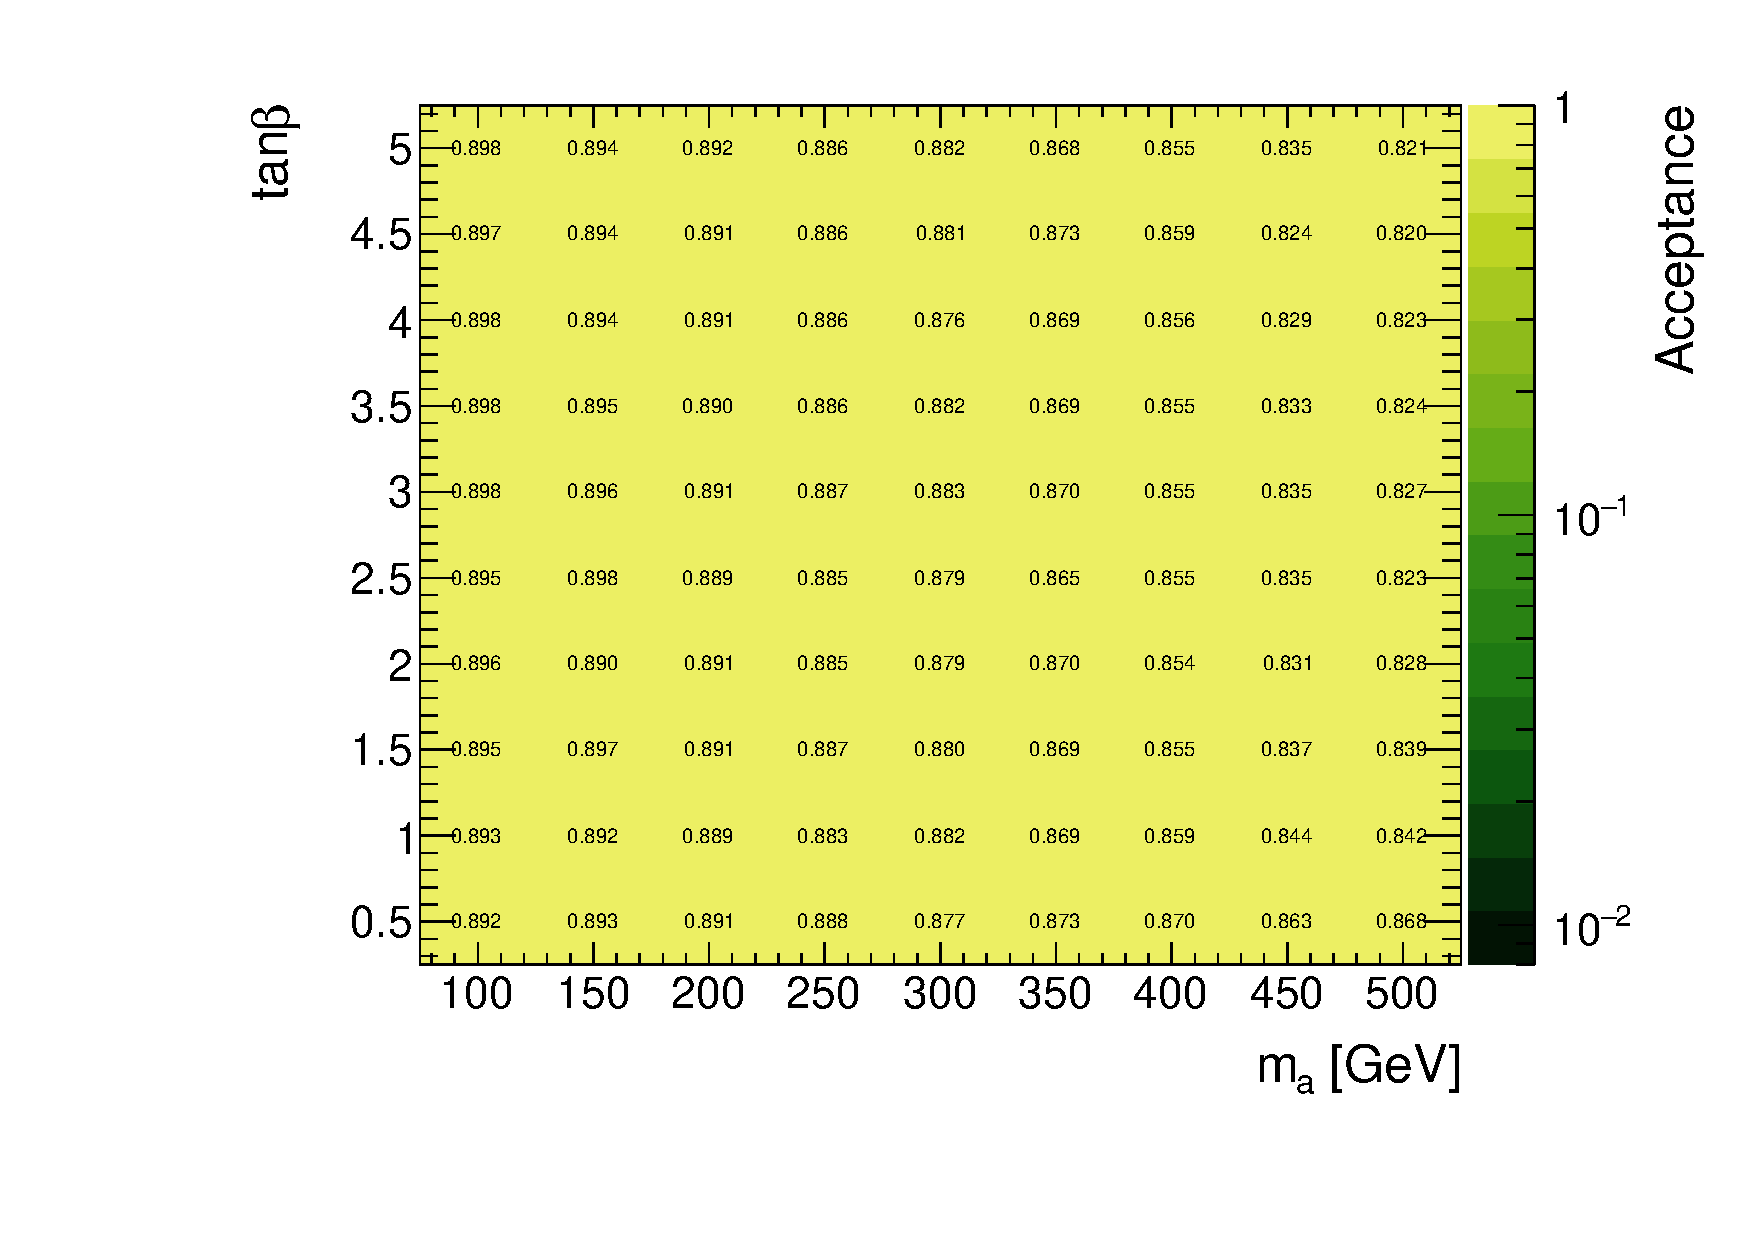
\includegraphics[width=0.45\textwidth]{texinputs/04_grid/figures/monoz/hadronic/grid_tanb_ma_incl_resl_acc.pdf}
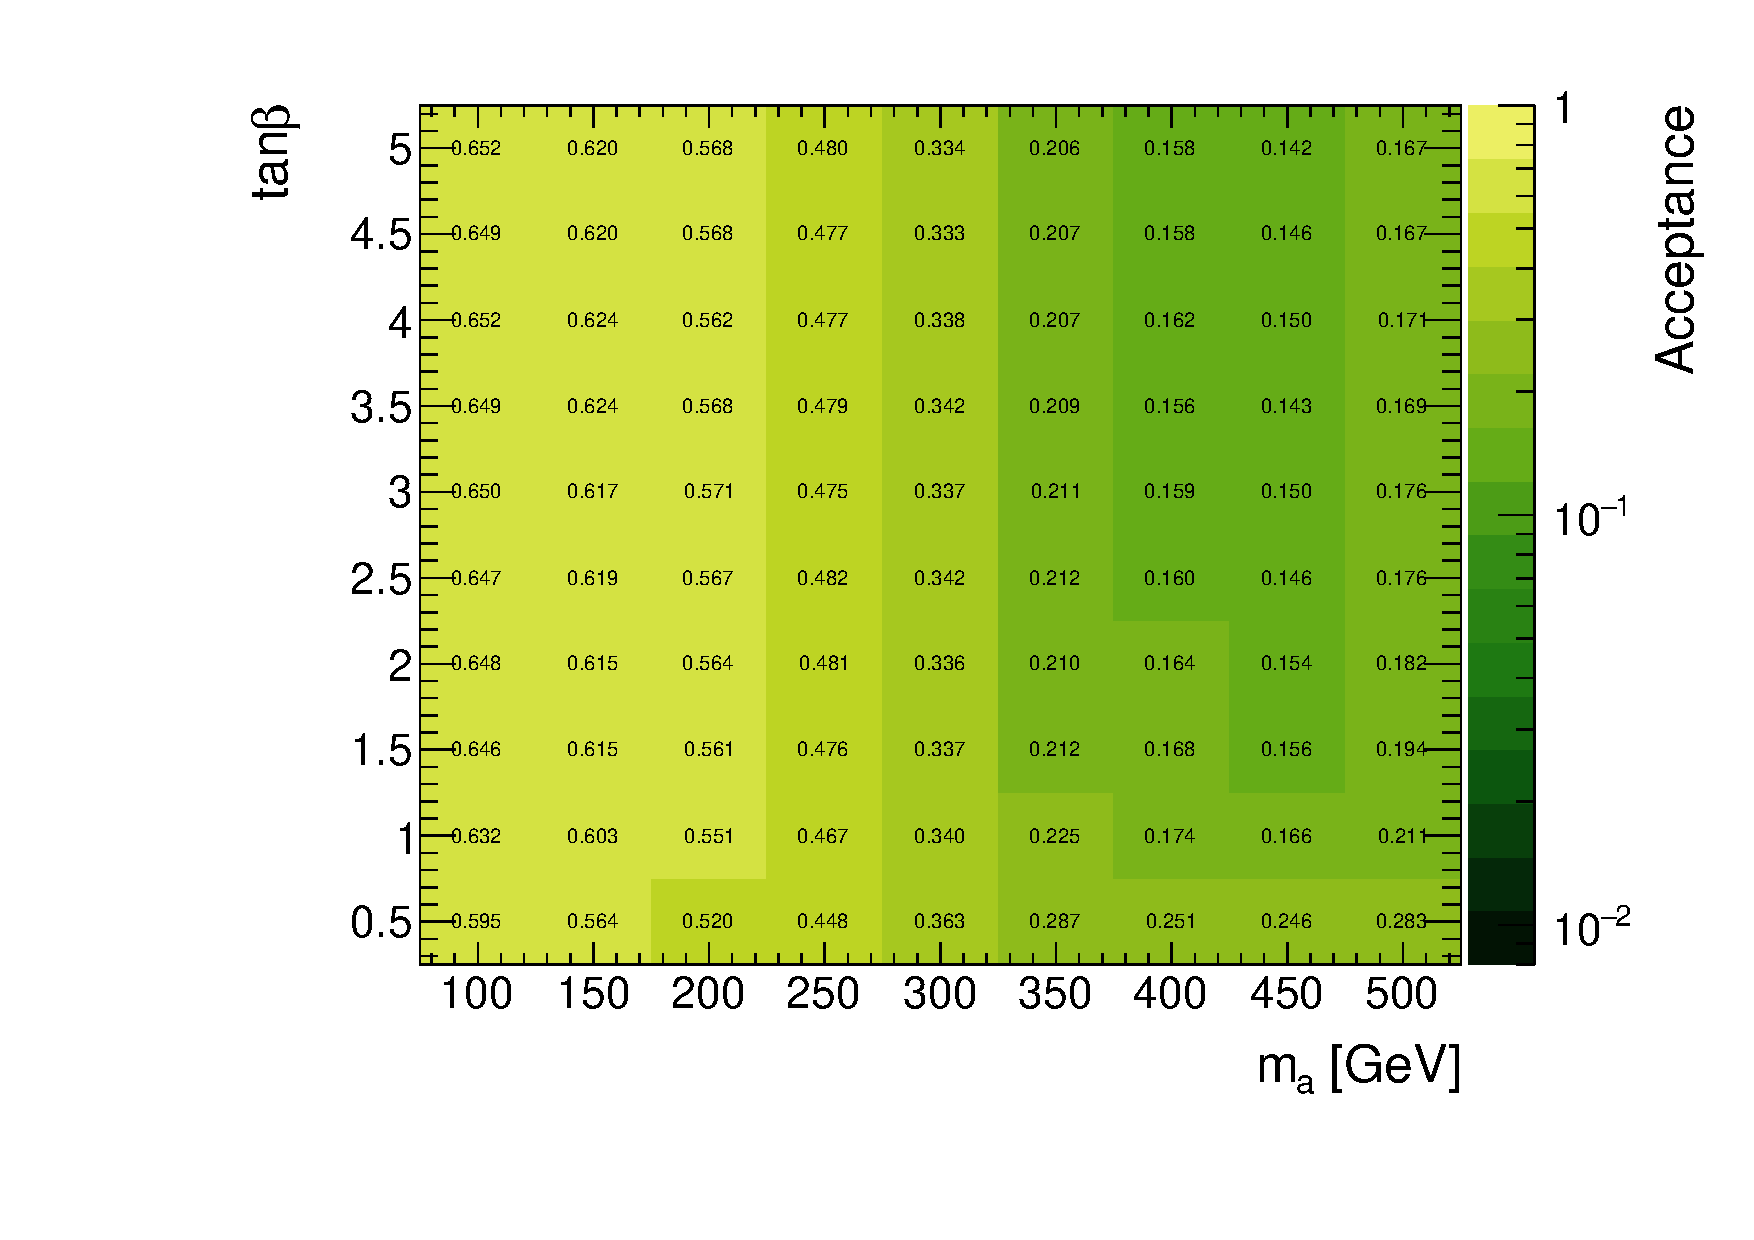
\includegraphics[width=0.45\textwidth]{texinputs/04_grid/figures/monoz/hadronic/grid_tanb_ma_incl_merged_acc.pdf}
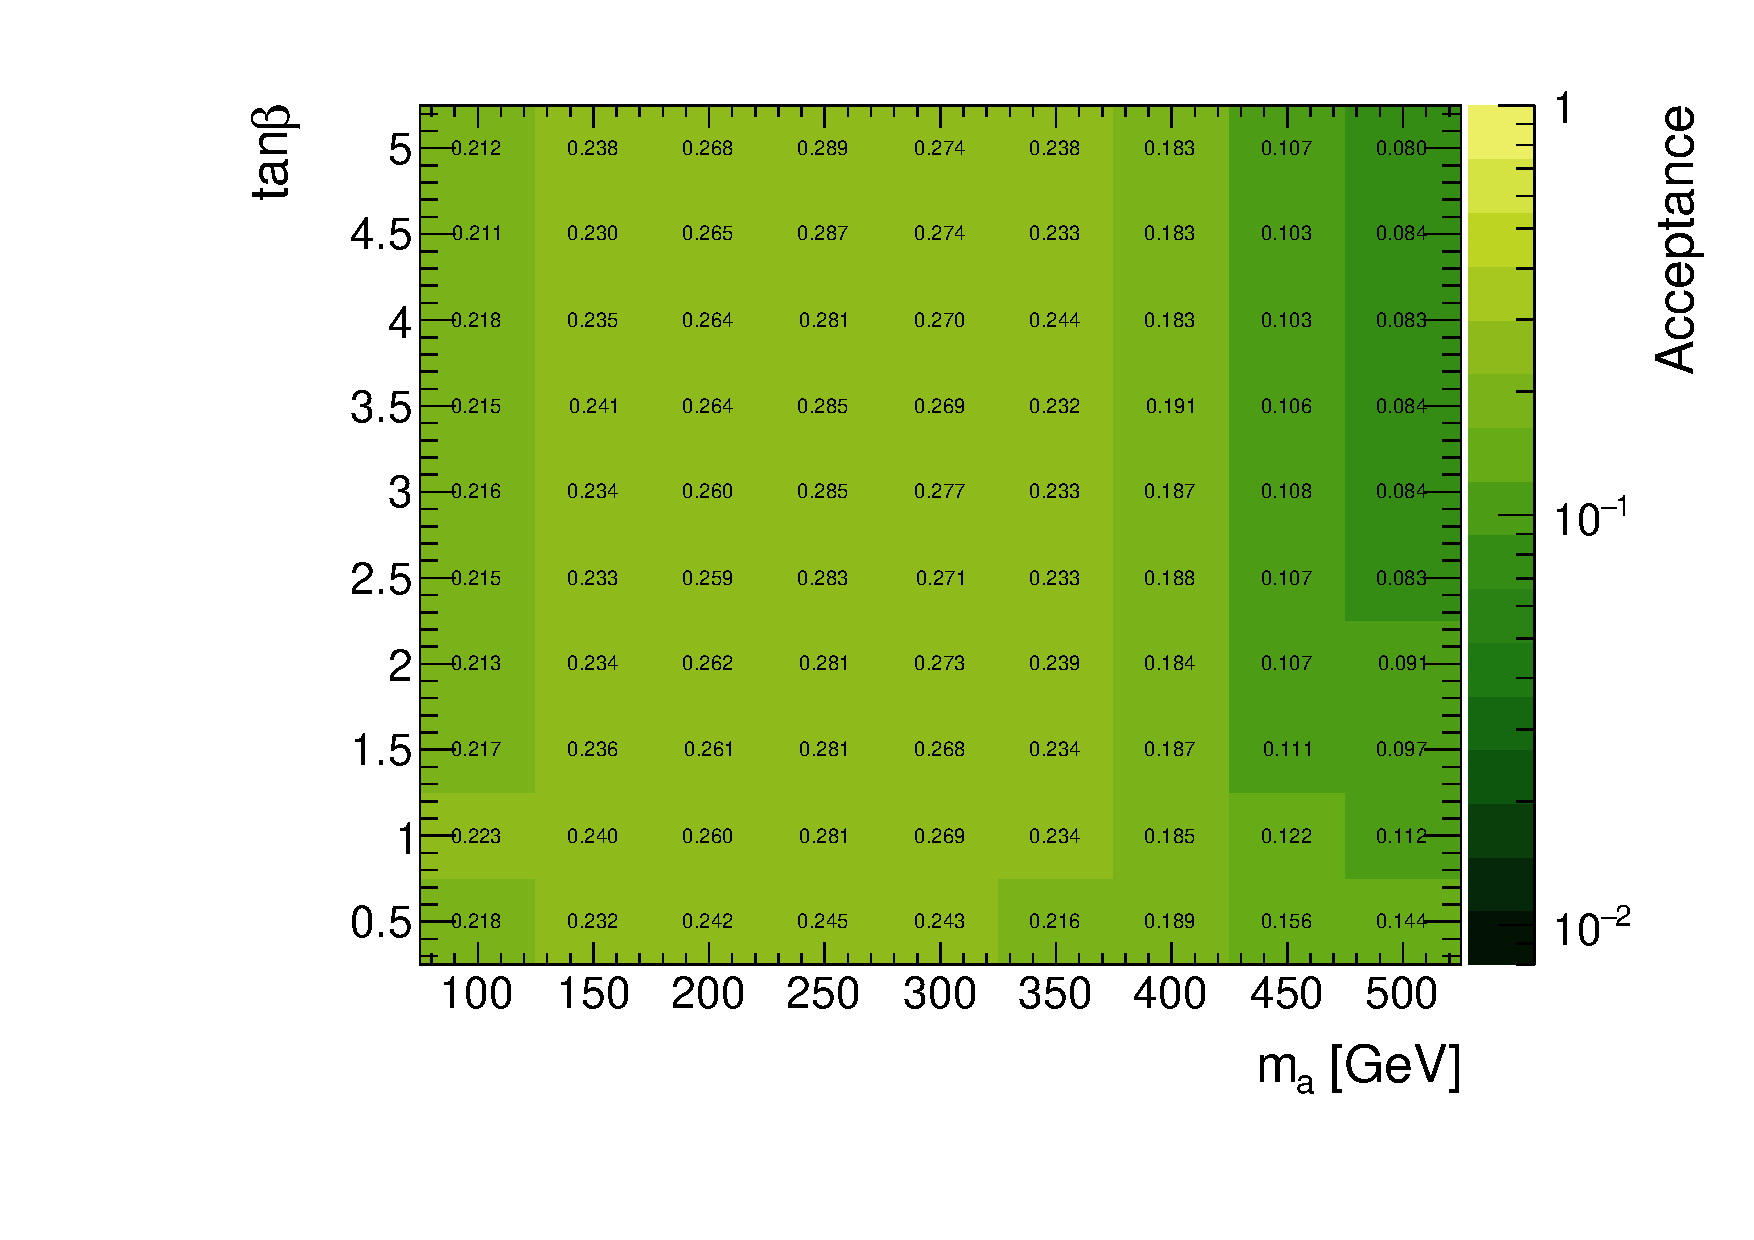
\includegraphics[width=0.45\textwidth]{texinputs/04_grid/figures/monoz/hadronic/grid_tanb_ma_resl_acc.pdf}
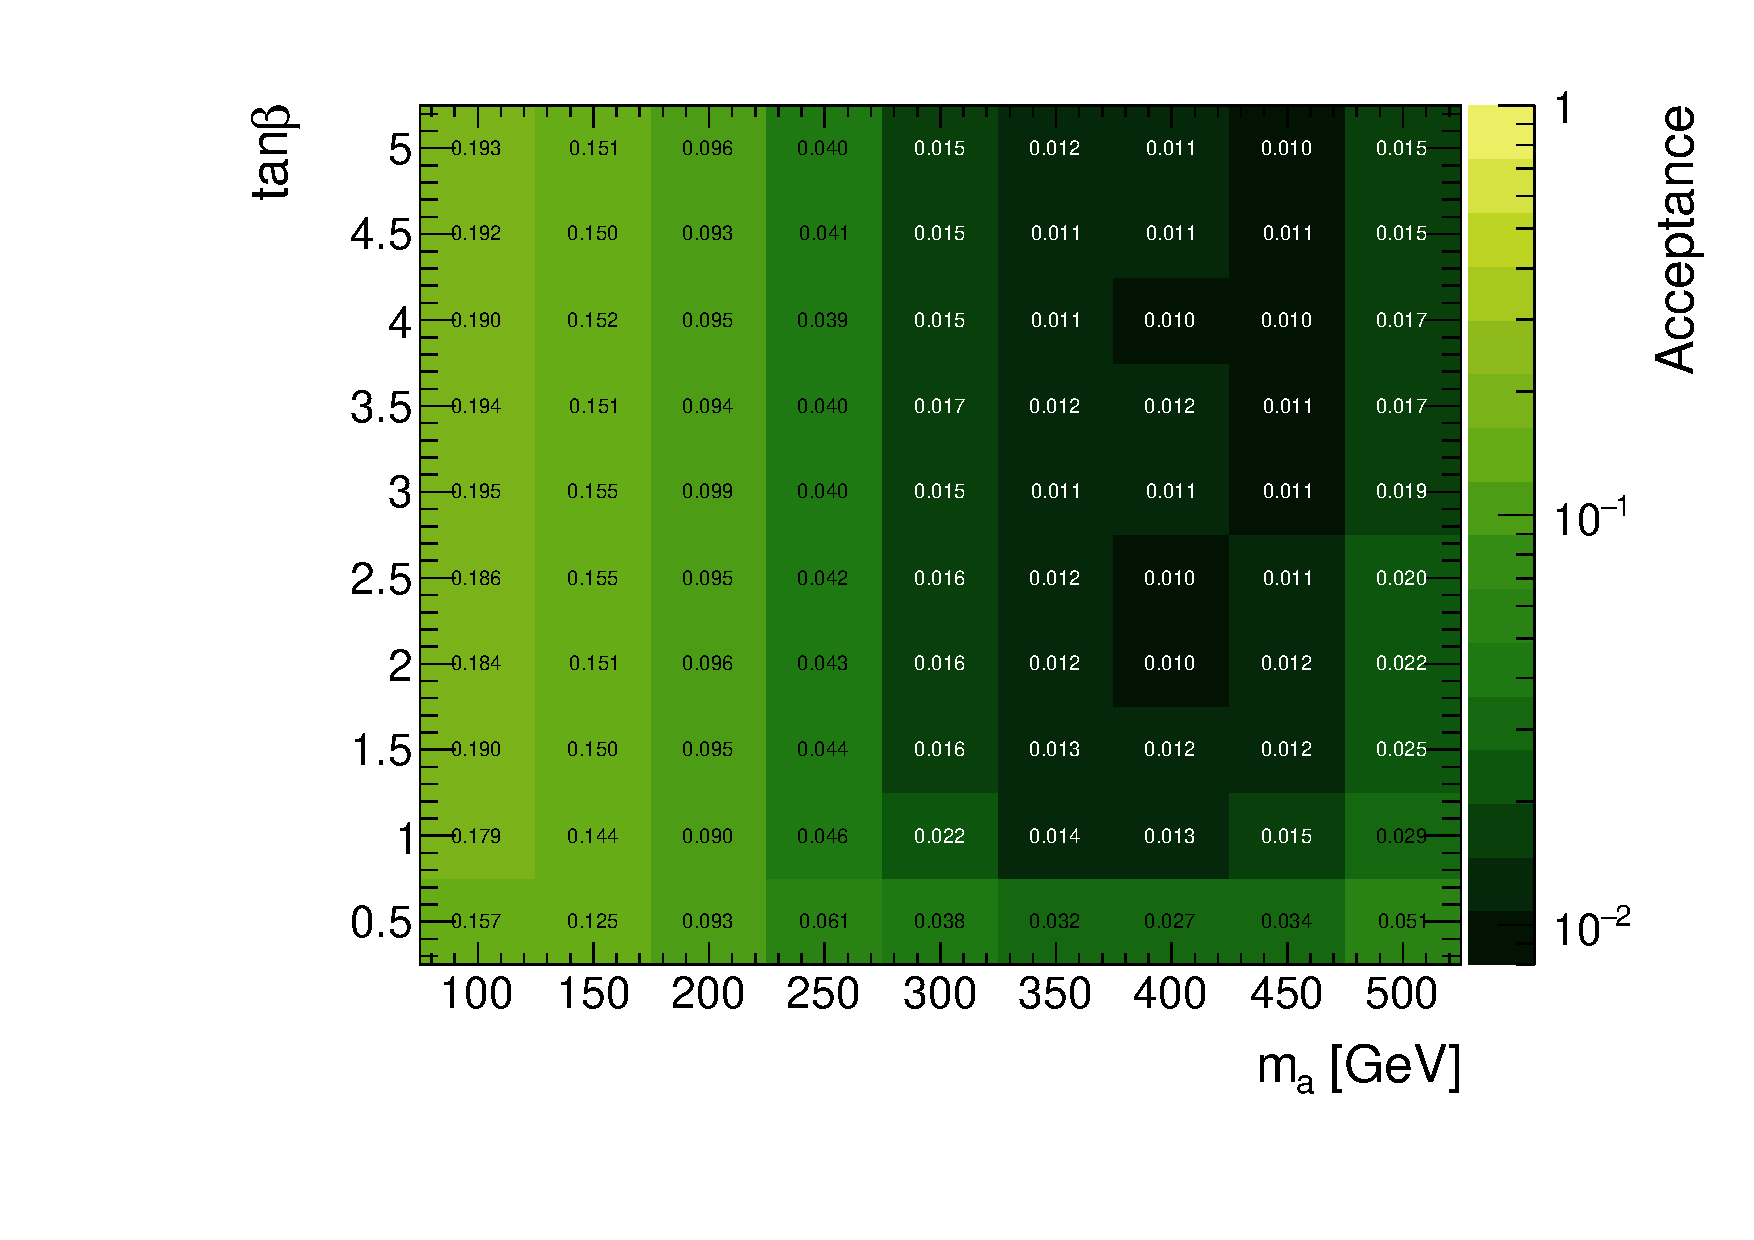
\includegraphics[width=0.45\textwidth]{texinputs/04_grid/figures/monoz/hadronic/grid_tanb_ma_merged_acc.pdf}
\caption{Acceptance for the inclusive (top) and final (bottom) selections for the mono-$Z$ hadronic events 
$pp \rightarrow Z(\to q\bar{q})\chi\overline{\chi}$ in the \ma vs $\tan\beta$ grid. 
Shown on the left (right) is the acceptance for the resolved (boosted) analysis selections. 
The \mA is fixed to 600~GeV.}
\label{fig:monozhad_acc_ma-tanb_grid}
\end{figure}

The signal acceptance in the \ma vs $\tan\beta$ space is shown in Fig.~\ref{fig:monozhad_acc_ma-tanb_grid}. 
The conventions used in Fig.~\ref{fig:monozhad_acc_ma-tanb_grid} are the same as those in 
Fig.~\ref{fig:monozhad_acc_ma-mA_grid}.
The signal acceptance is rather independent of $\tan\beta$ except at low $\tan\beta$ region; the acceptance 
tends to be slightly lower at $\tan\beta<1$ than at $>1$ for $\ma<\sim250$~GeV while it's opposite for 
$\ma>\sim250$~GeV. The acceptance decreases with increasing \ma because the \MET spectrum becomes 
softer with \ma, as shown in Fig.~\ref{fig:monozhad_kin_inc_fixed_mA}.


\begin{figure}
\centering
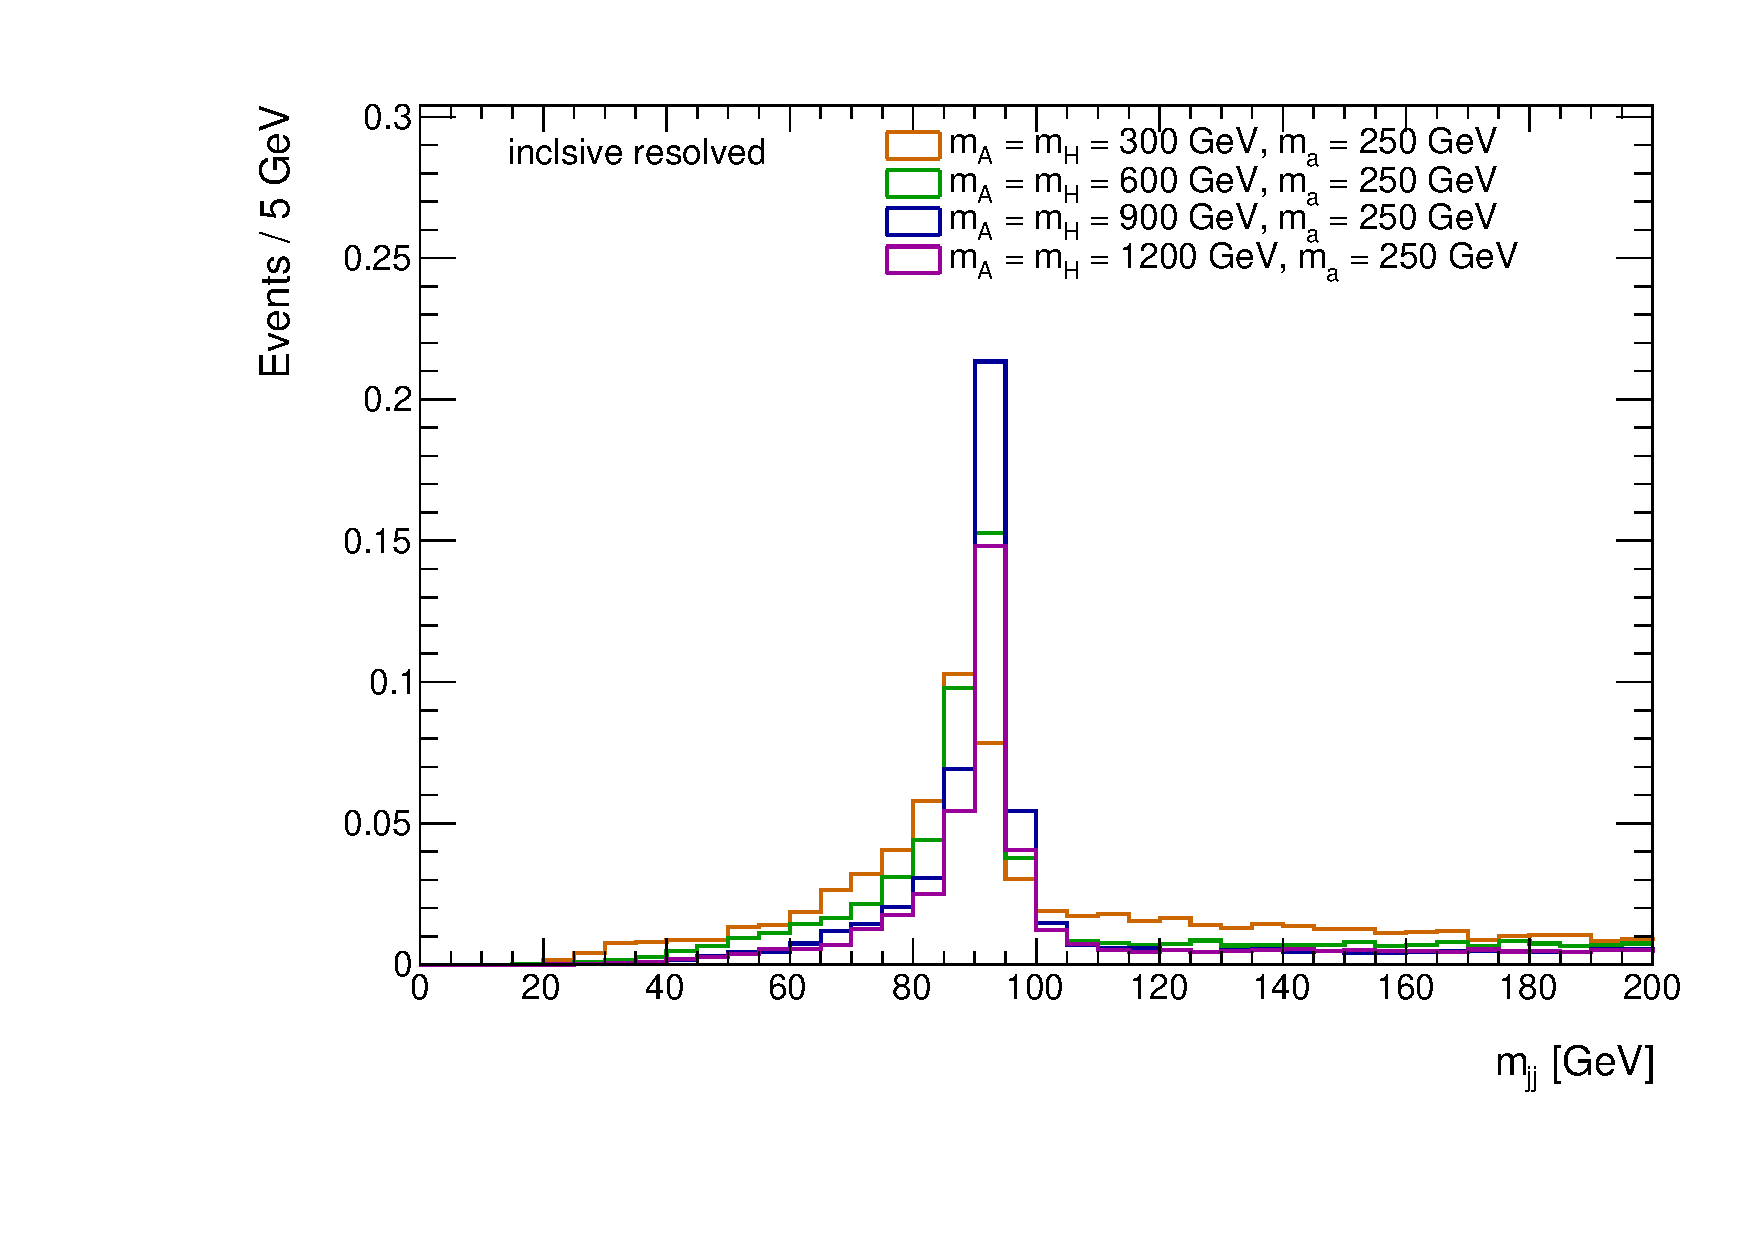
\includegraphics[width=0.45\textwidth]{texinputs/04_grid/figures/monoz/hadronic/ma250_incl_resl_MJJ_linear.pdf}
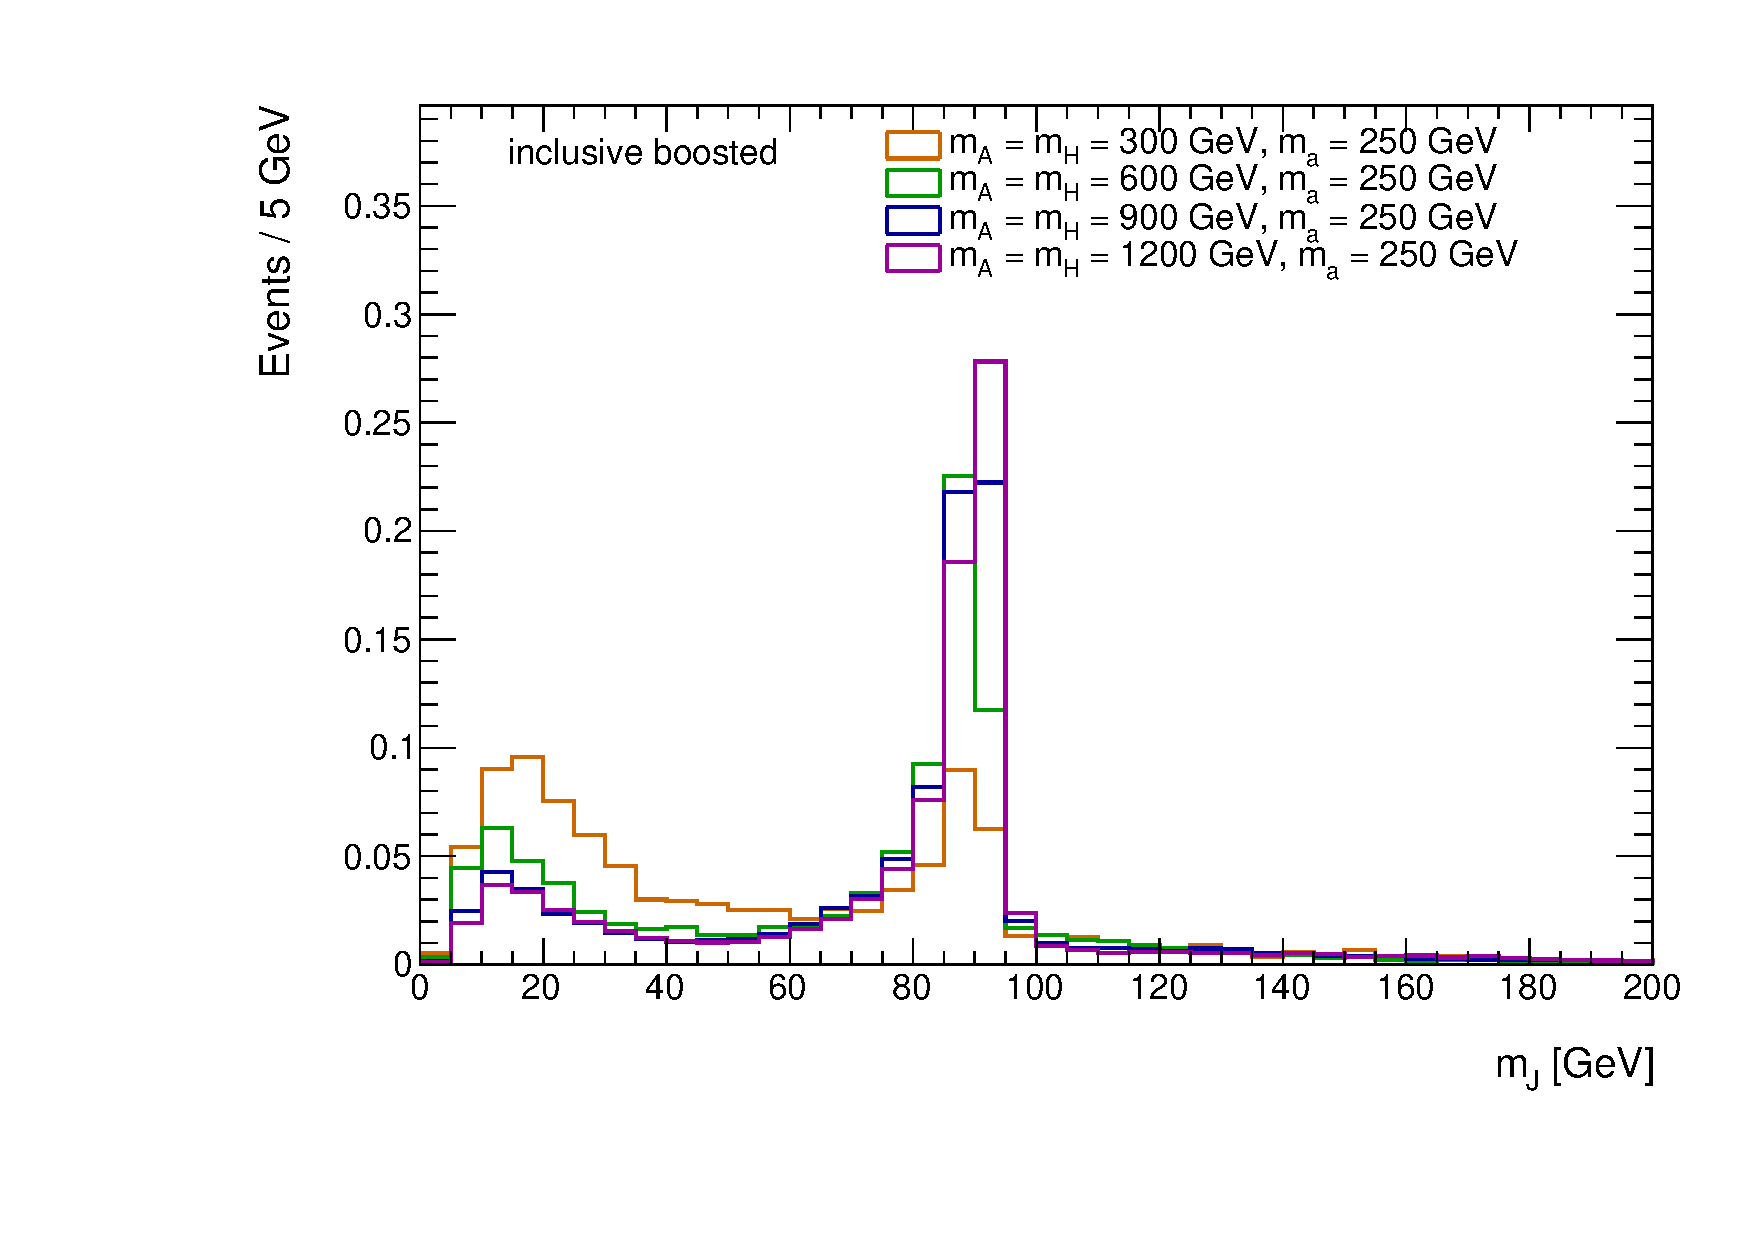
\includegraphics[width=0.45\textwidth]{texinputs/04_grid/figures/monoz/hadronic/ma250_incl_merged_MFatJ1_linear.pdf}
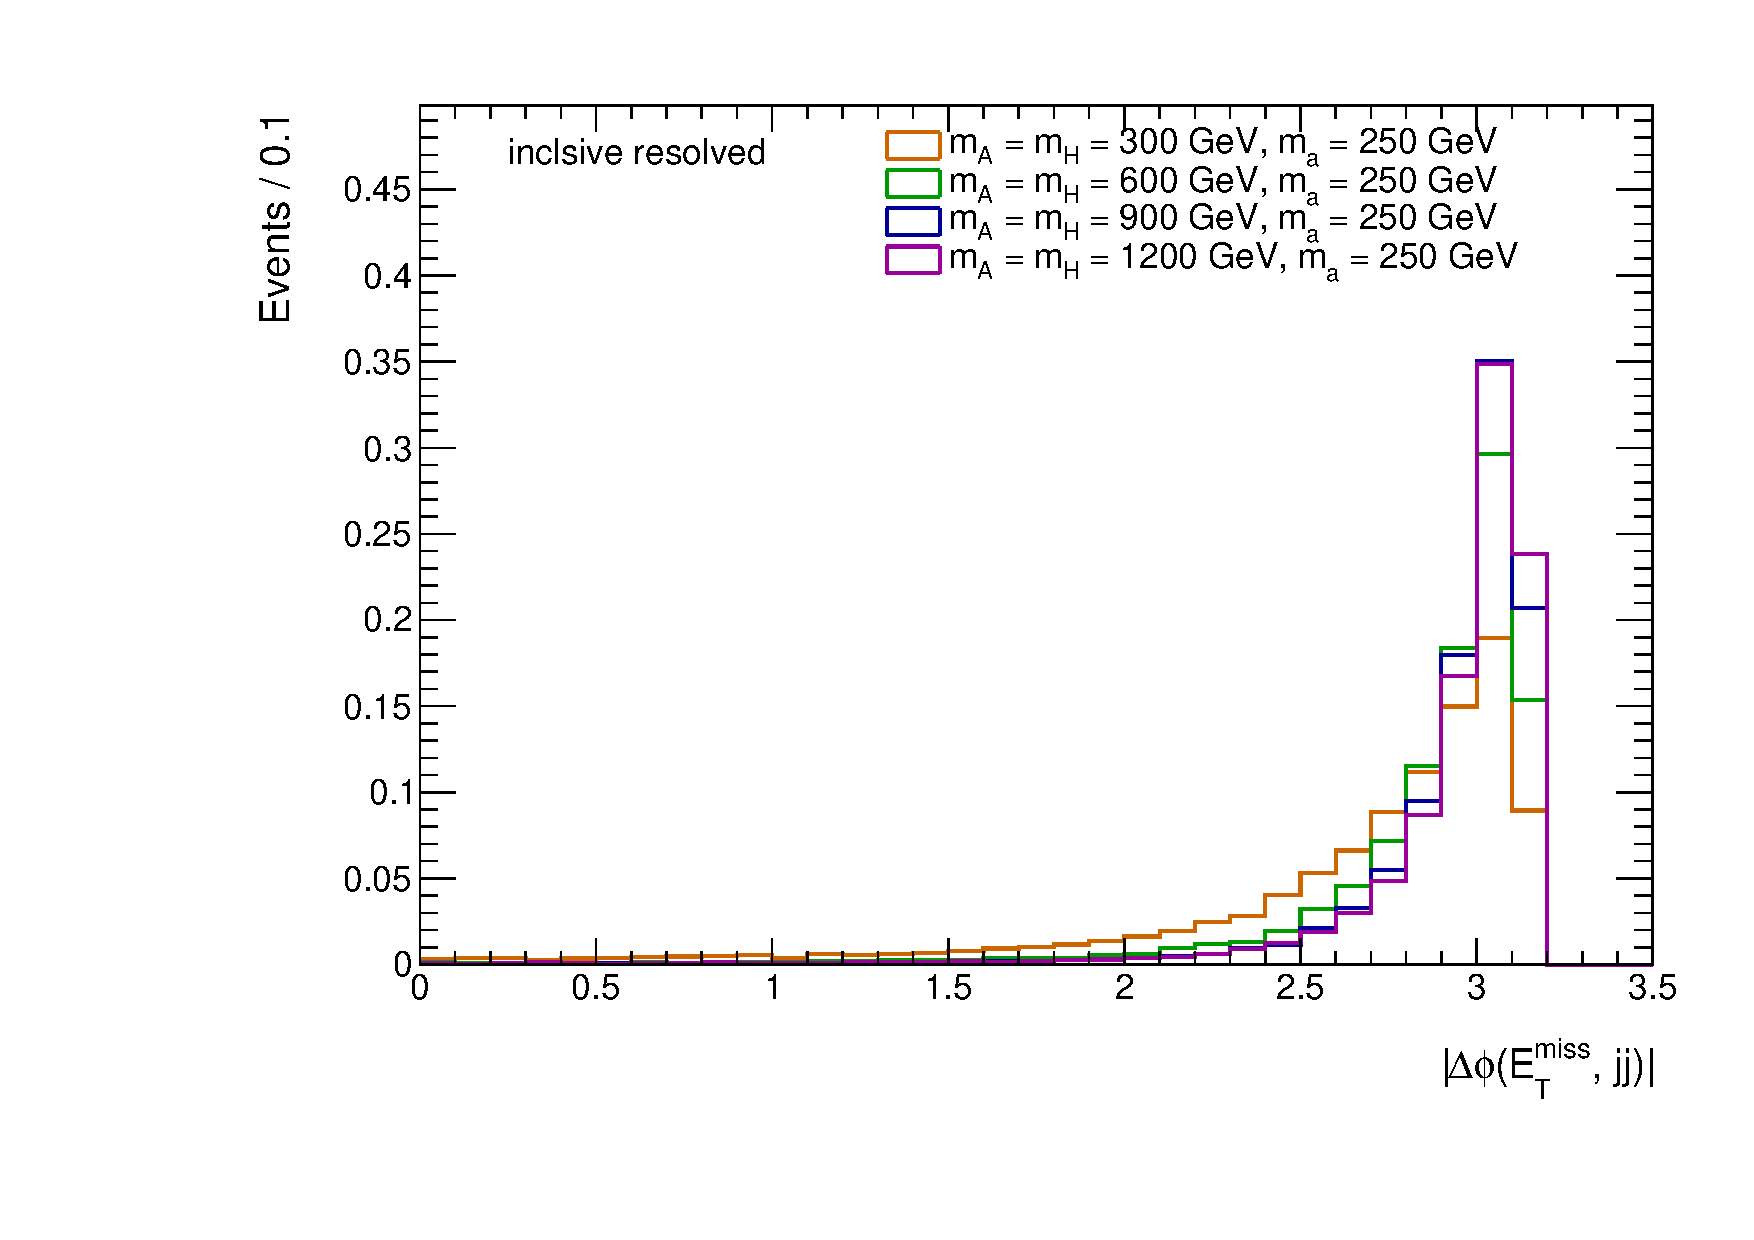
\includegraphics[width=0.45\textwidth]{texinputs/04_grid/figures/monoz/hadronic/ma250_incl_resl_dPhiMETJJ_linear.pdf}
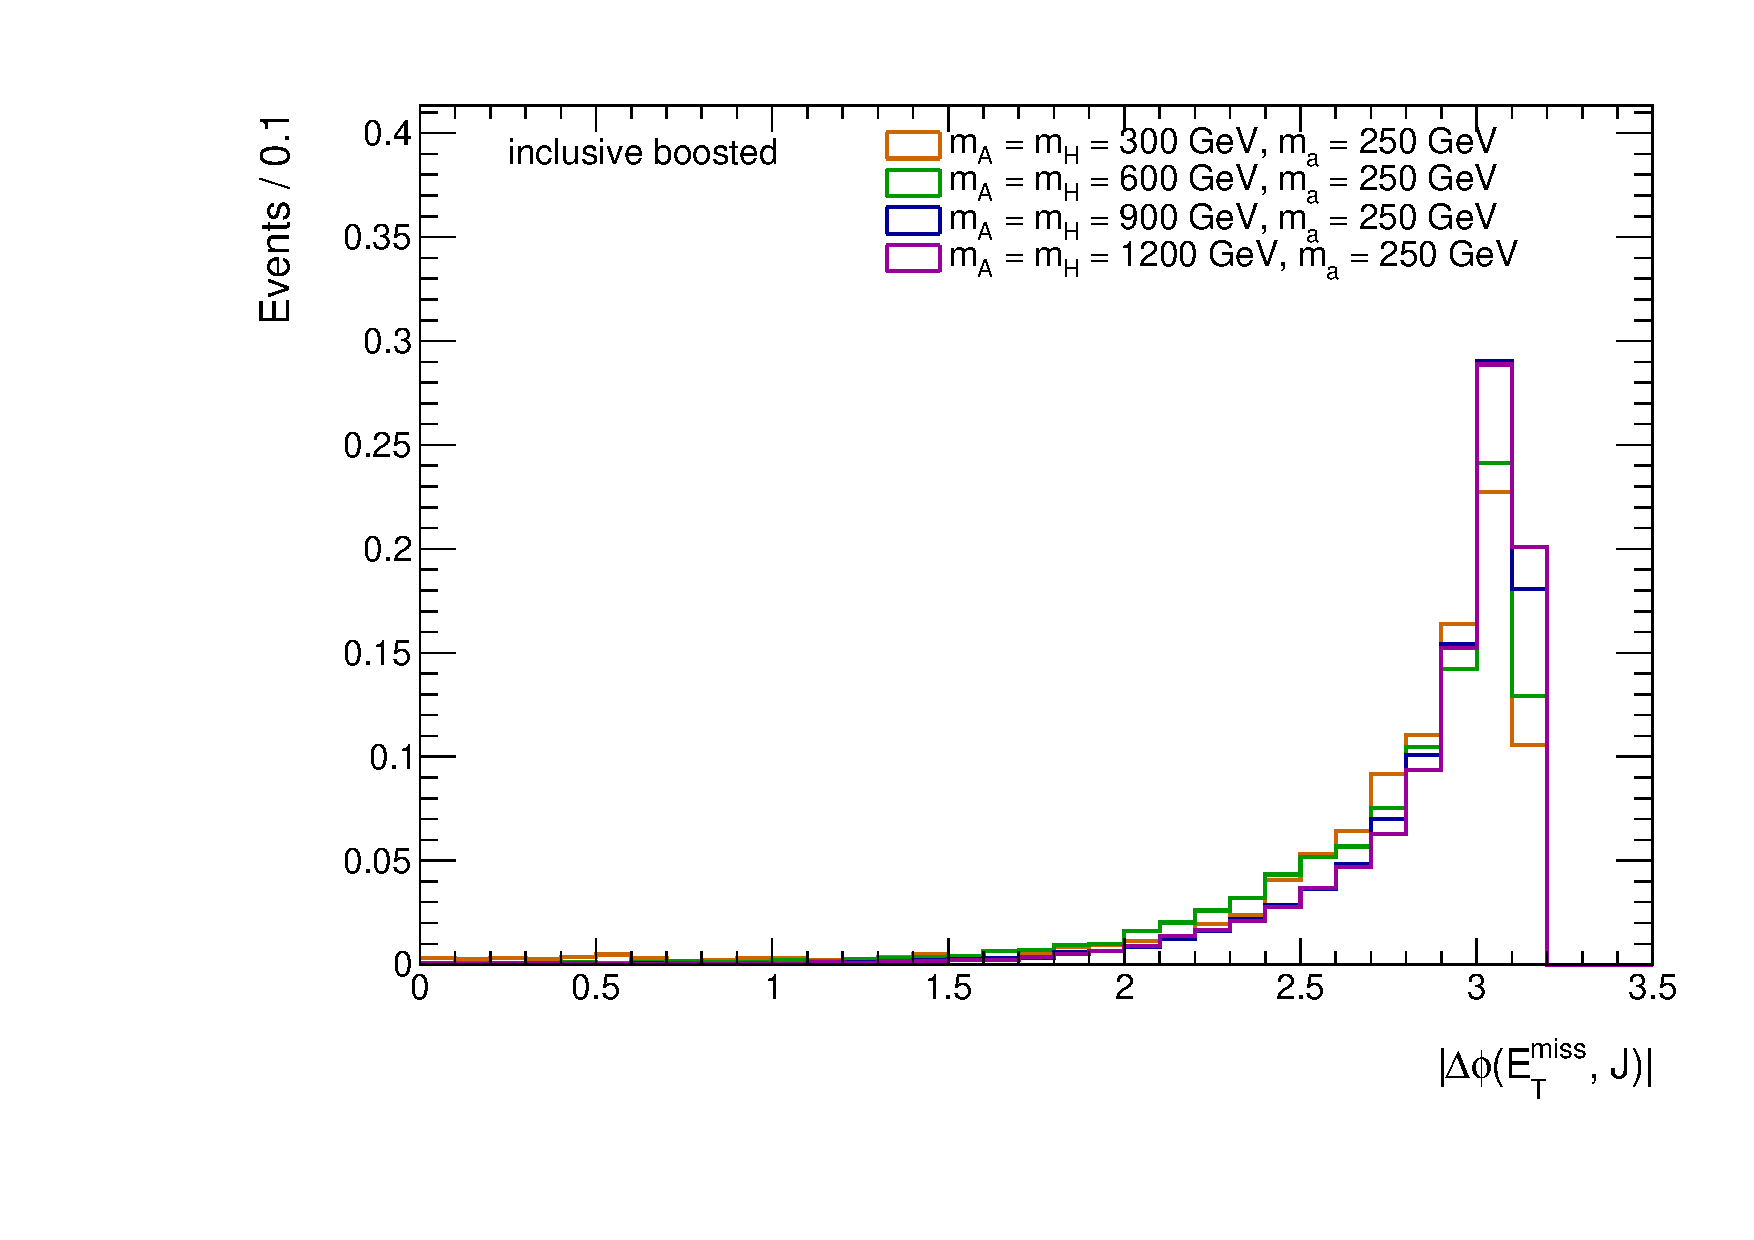
\includegraphics[width=0.45\textwidth]{texinputs/04_grid/figures/monoz/hadronic/ma250_incl_merged_dPhiMETJ_linear.pdf}
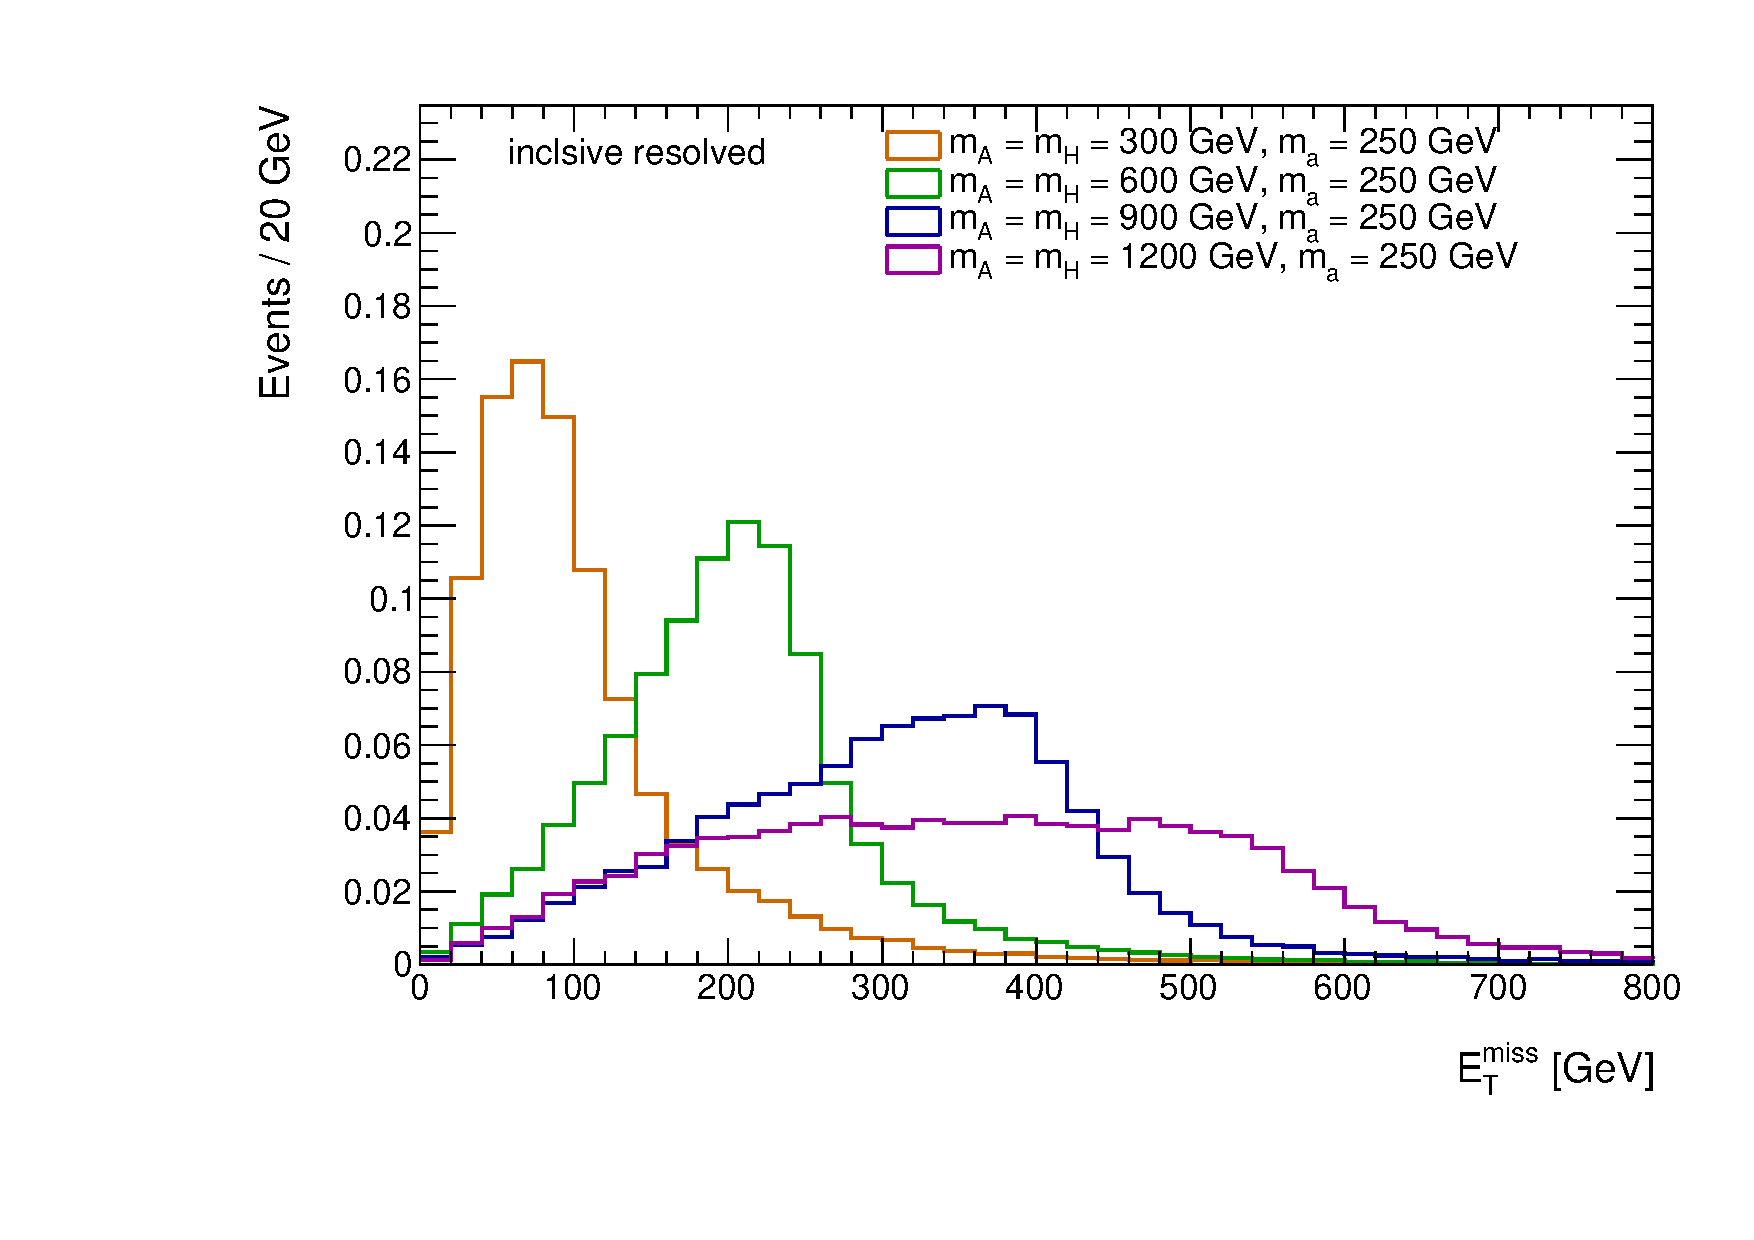
\includegraphics[width=0.45\textwidth]{texinputs/04_grid/figures/monoz/hadronic/ma250_incl_resl_MET_linear.pdf}
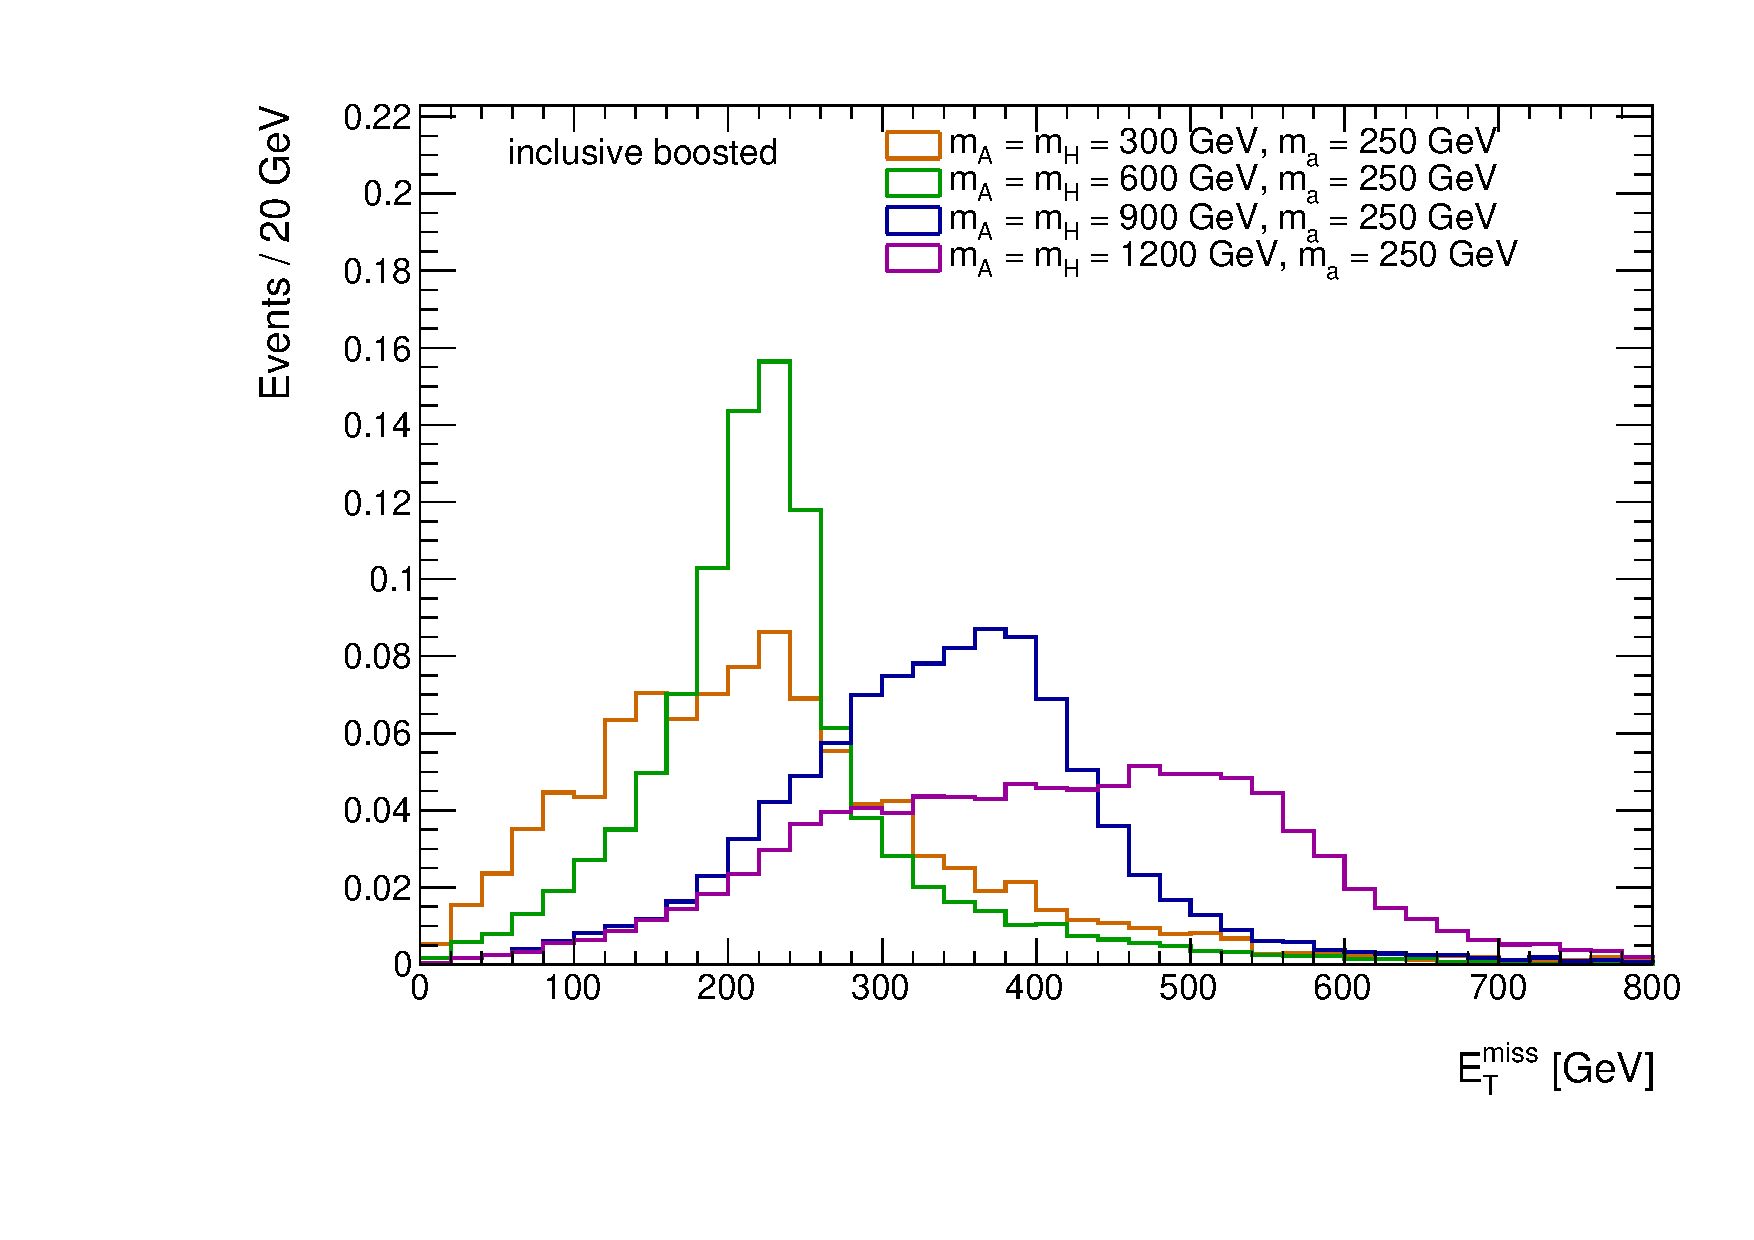
\includegraphics[width=0.45\textwidth]{texinputs/04_grid/figures/monoz/hadronic/ma250_incl_merged_MET_linear.pdf}
\caption{Dijet mass (top), $\Delta\Phi(jj, \MET)$ (middle) and $\MET$ (bottom) distributions 
after applying the inclusive selections in the resolved analysis are shown on the left side. Large-radius 
jet mass (top), $\Delta\Phi(J, \MET)$ (middle) and $\MET$ (bottom) distributions 
after applying the inclusive selections in the boosted analysis are shown on the right side. 
The signal masses are chosen to be \mA = 300, 600, 900 and 1200~GeV with the fixed \ma = 250~GeV.}
\label{fig:monozhad_kin_inc_fixed_ma}
\end{figure}

\begin{figure}
\centering
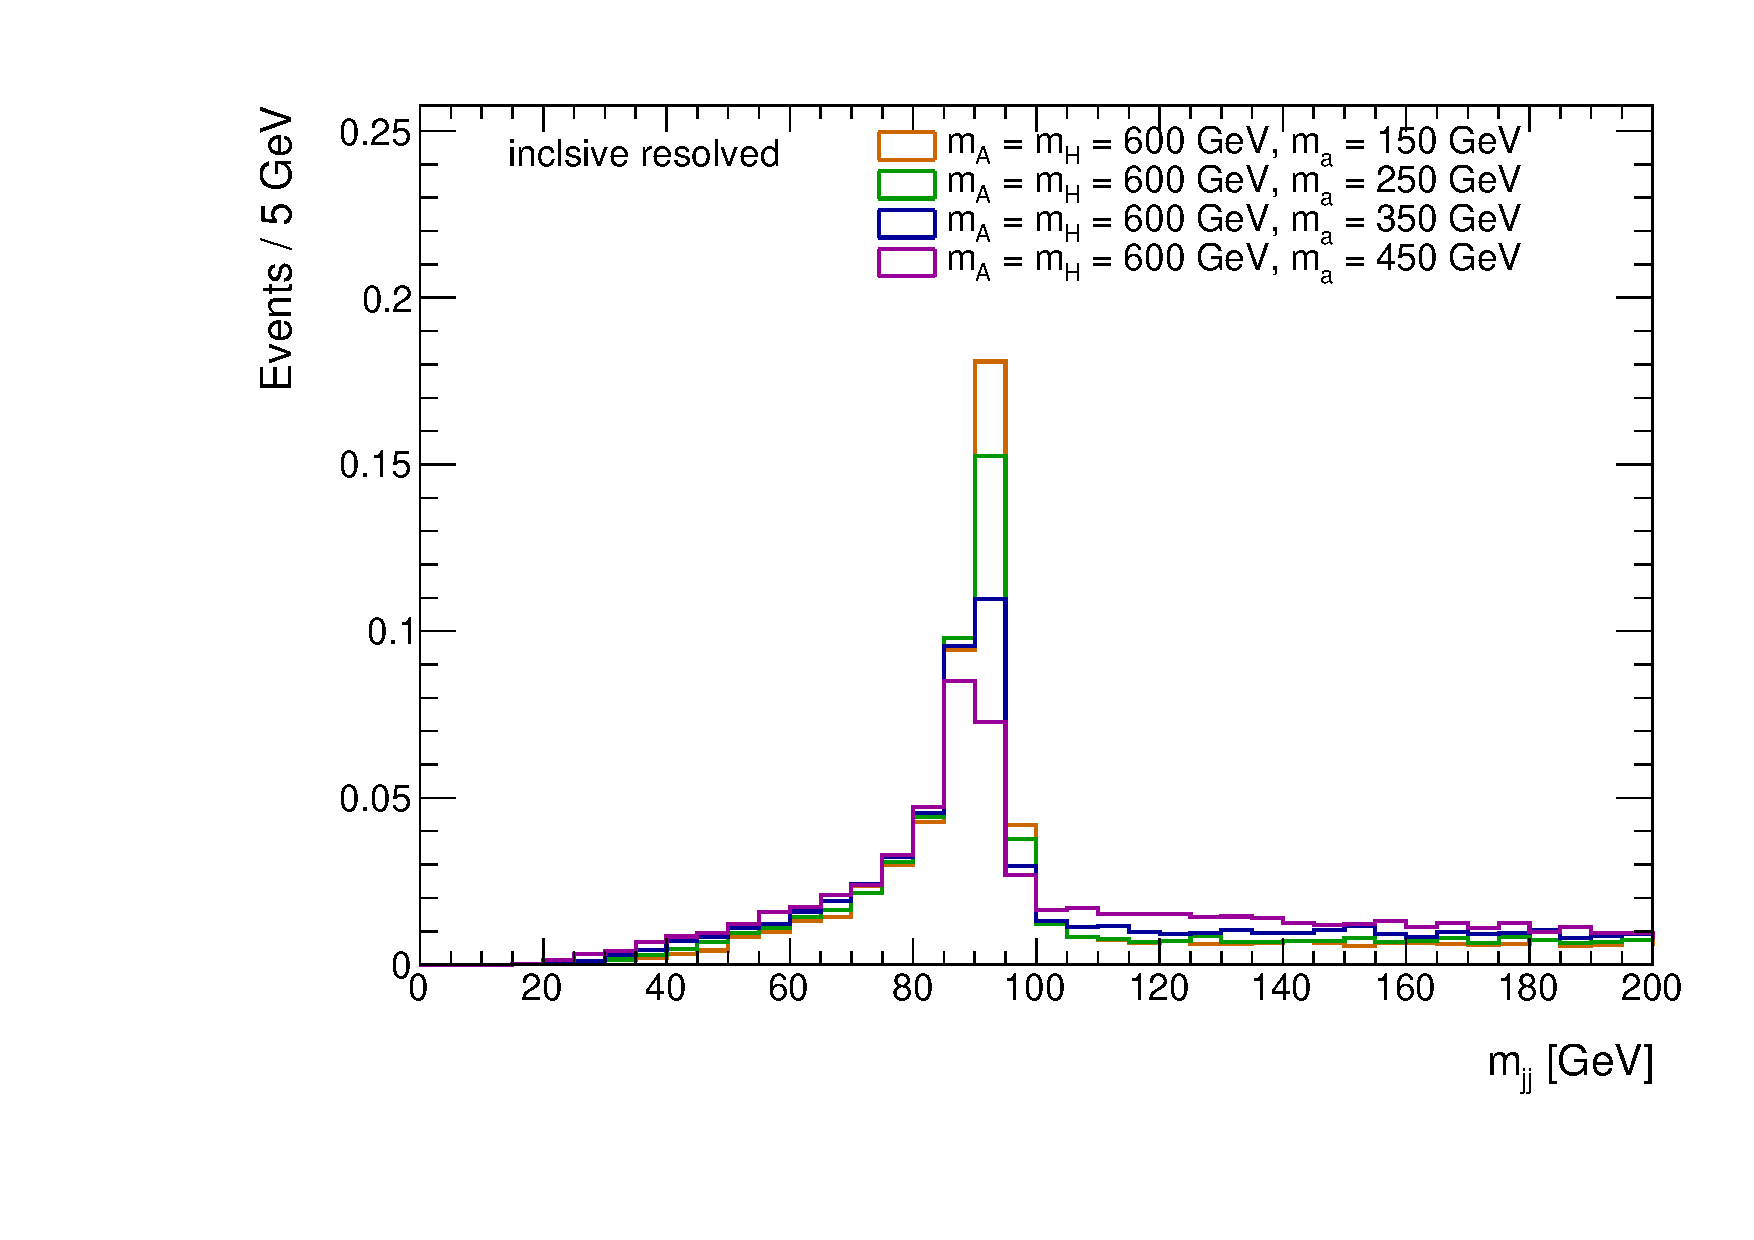
\includegraphics[width=0.45\textwidth]{texinputs/04_grid/figures/monoz/hadronic/mA600_incl_resl_MJJ_linear.pdf}
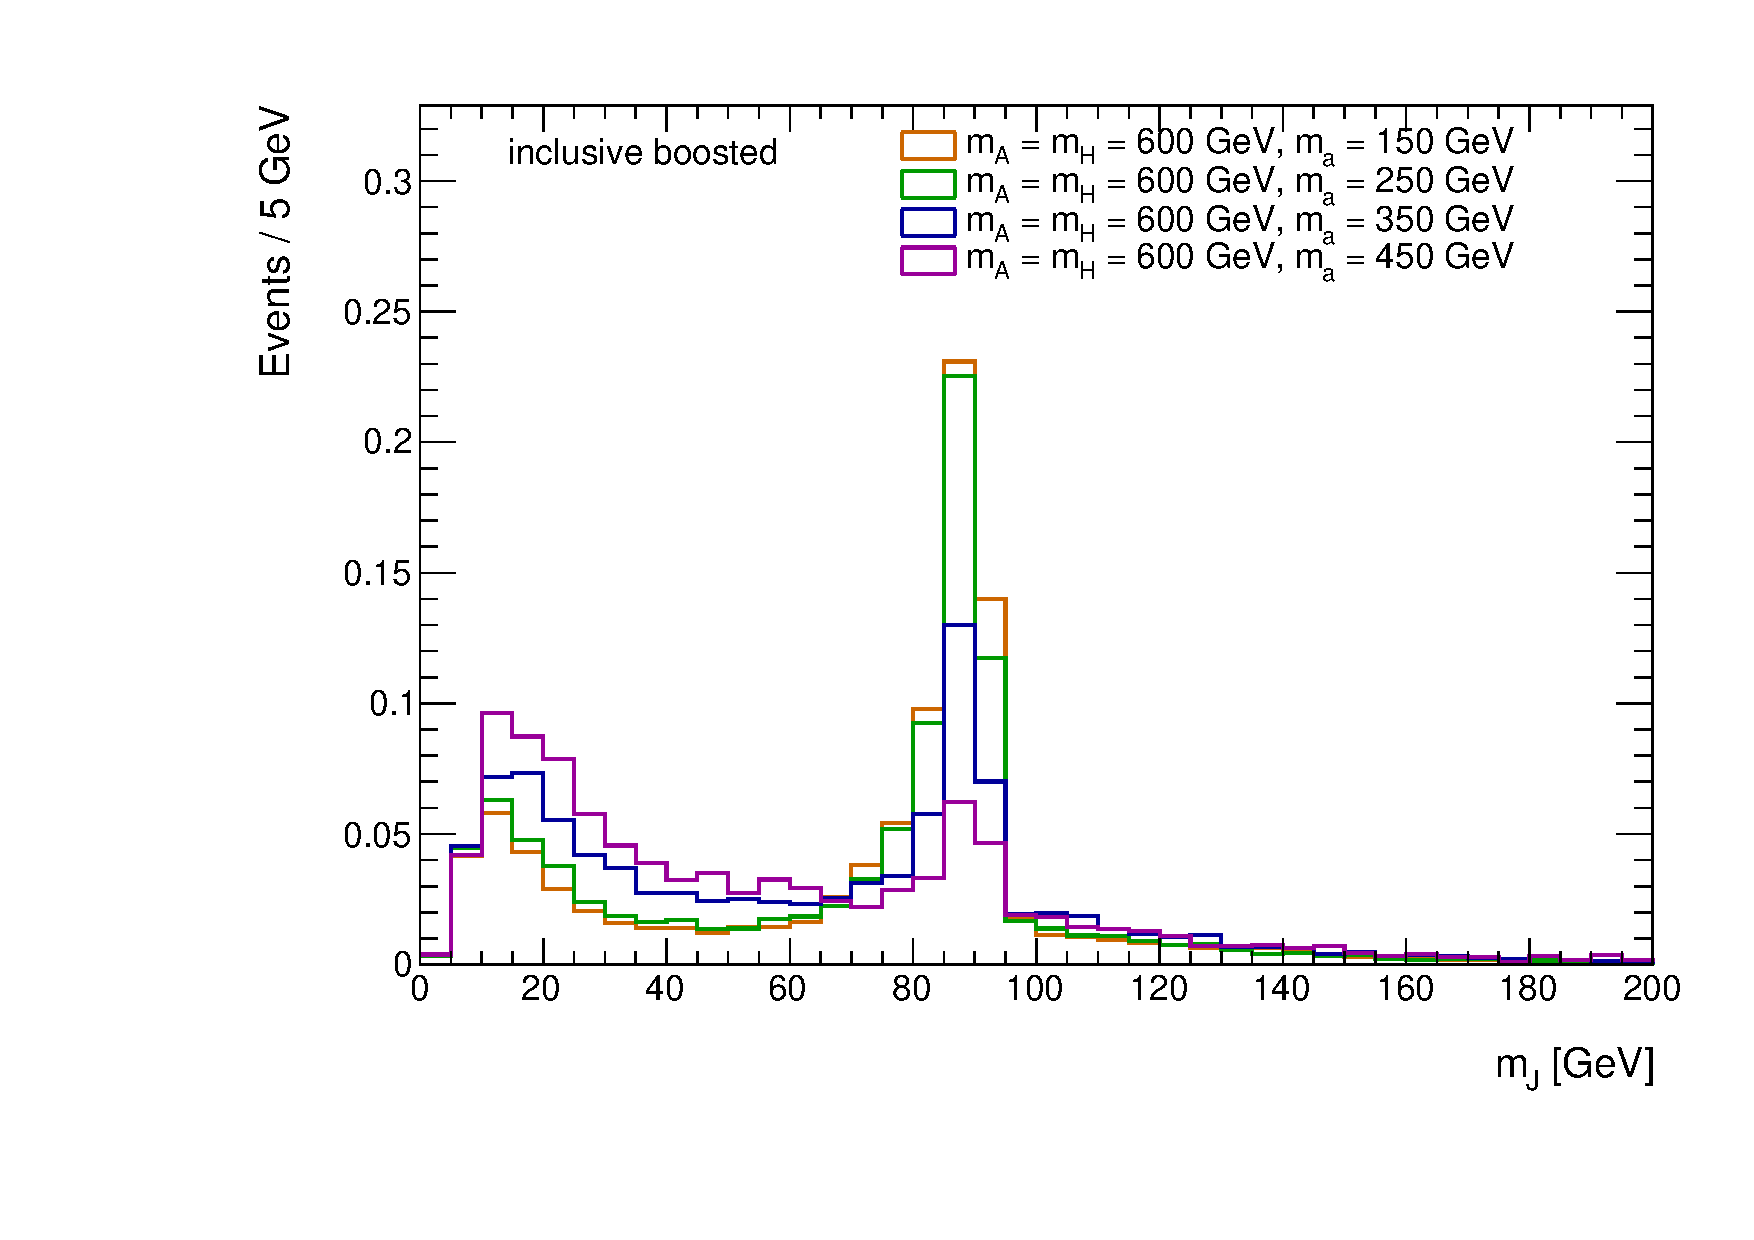
\includegraphics[width=0.45\textwidth]{texinputs/04_grid/figures/monoz/hadronic/mA600_incl_merged_MFatJ1_linear.pdf}
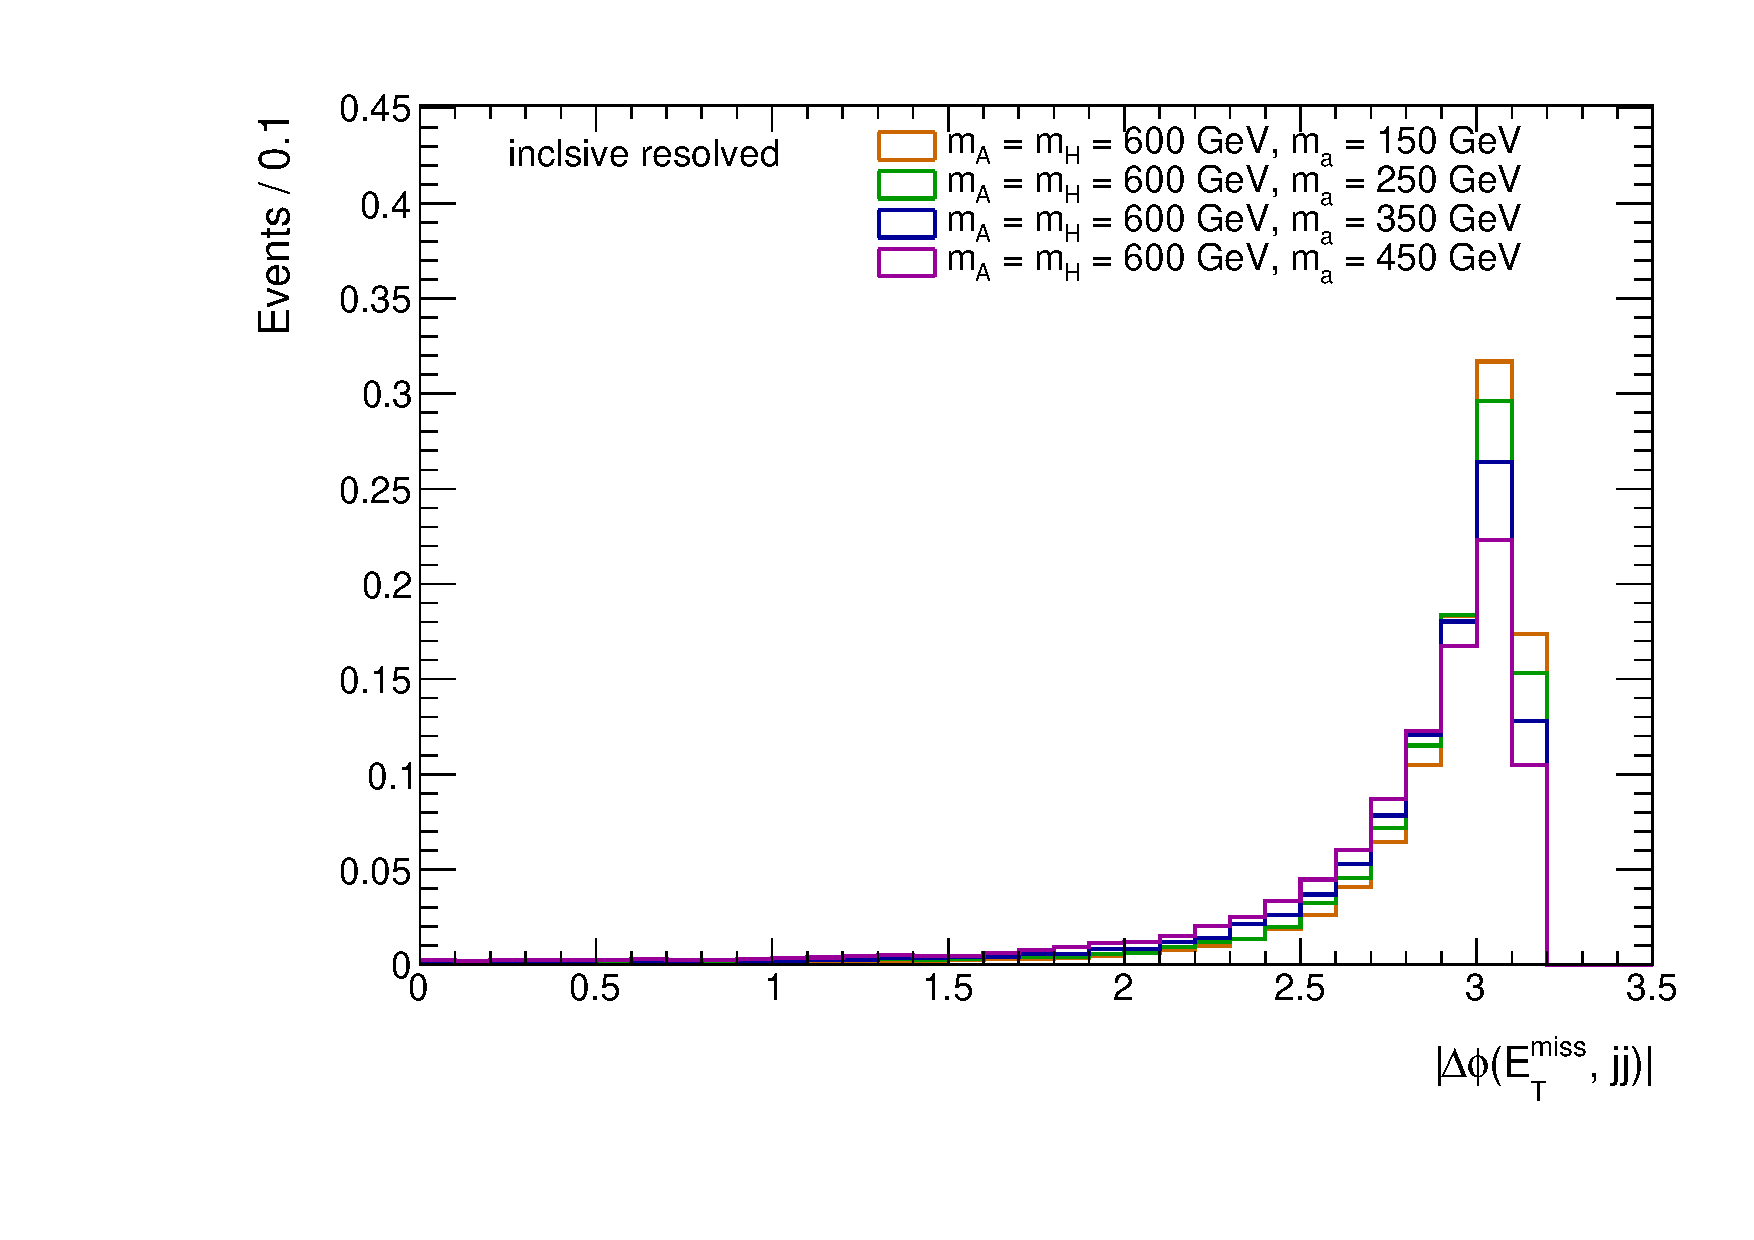
\includegraphics[width=0.45\textwidth]{texinputs/04_grid/figures/monoz/hadronic/mA600_incl_resl_dPhiMETJJ_linear.pdf}
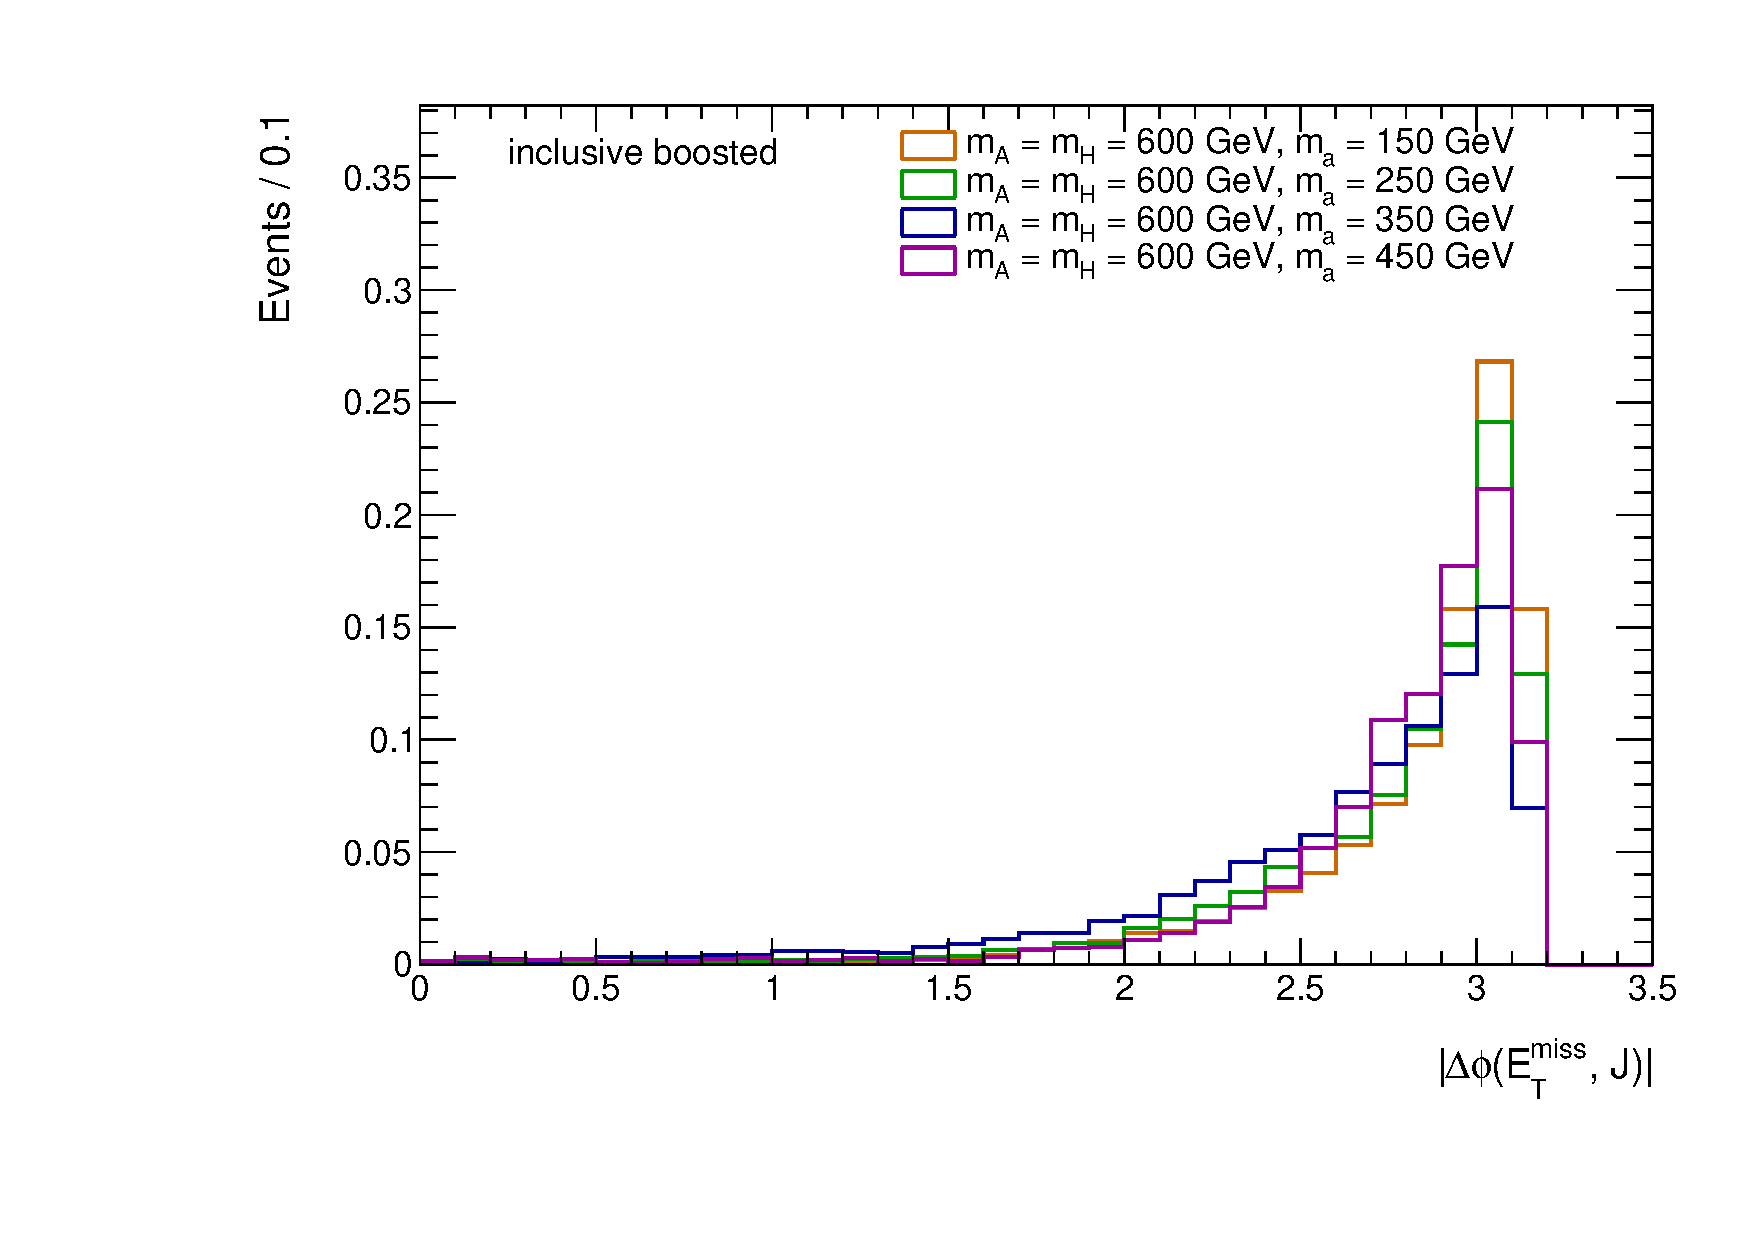
\includegraphics[width=0.45\textwidth]{texinputs/04_grid/figures/monoz/hadronic/mA600_incl_merged_dPhiMETJ_linear.pdf}
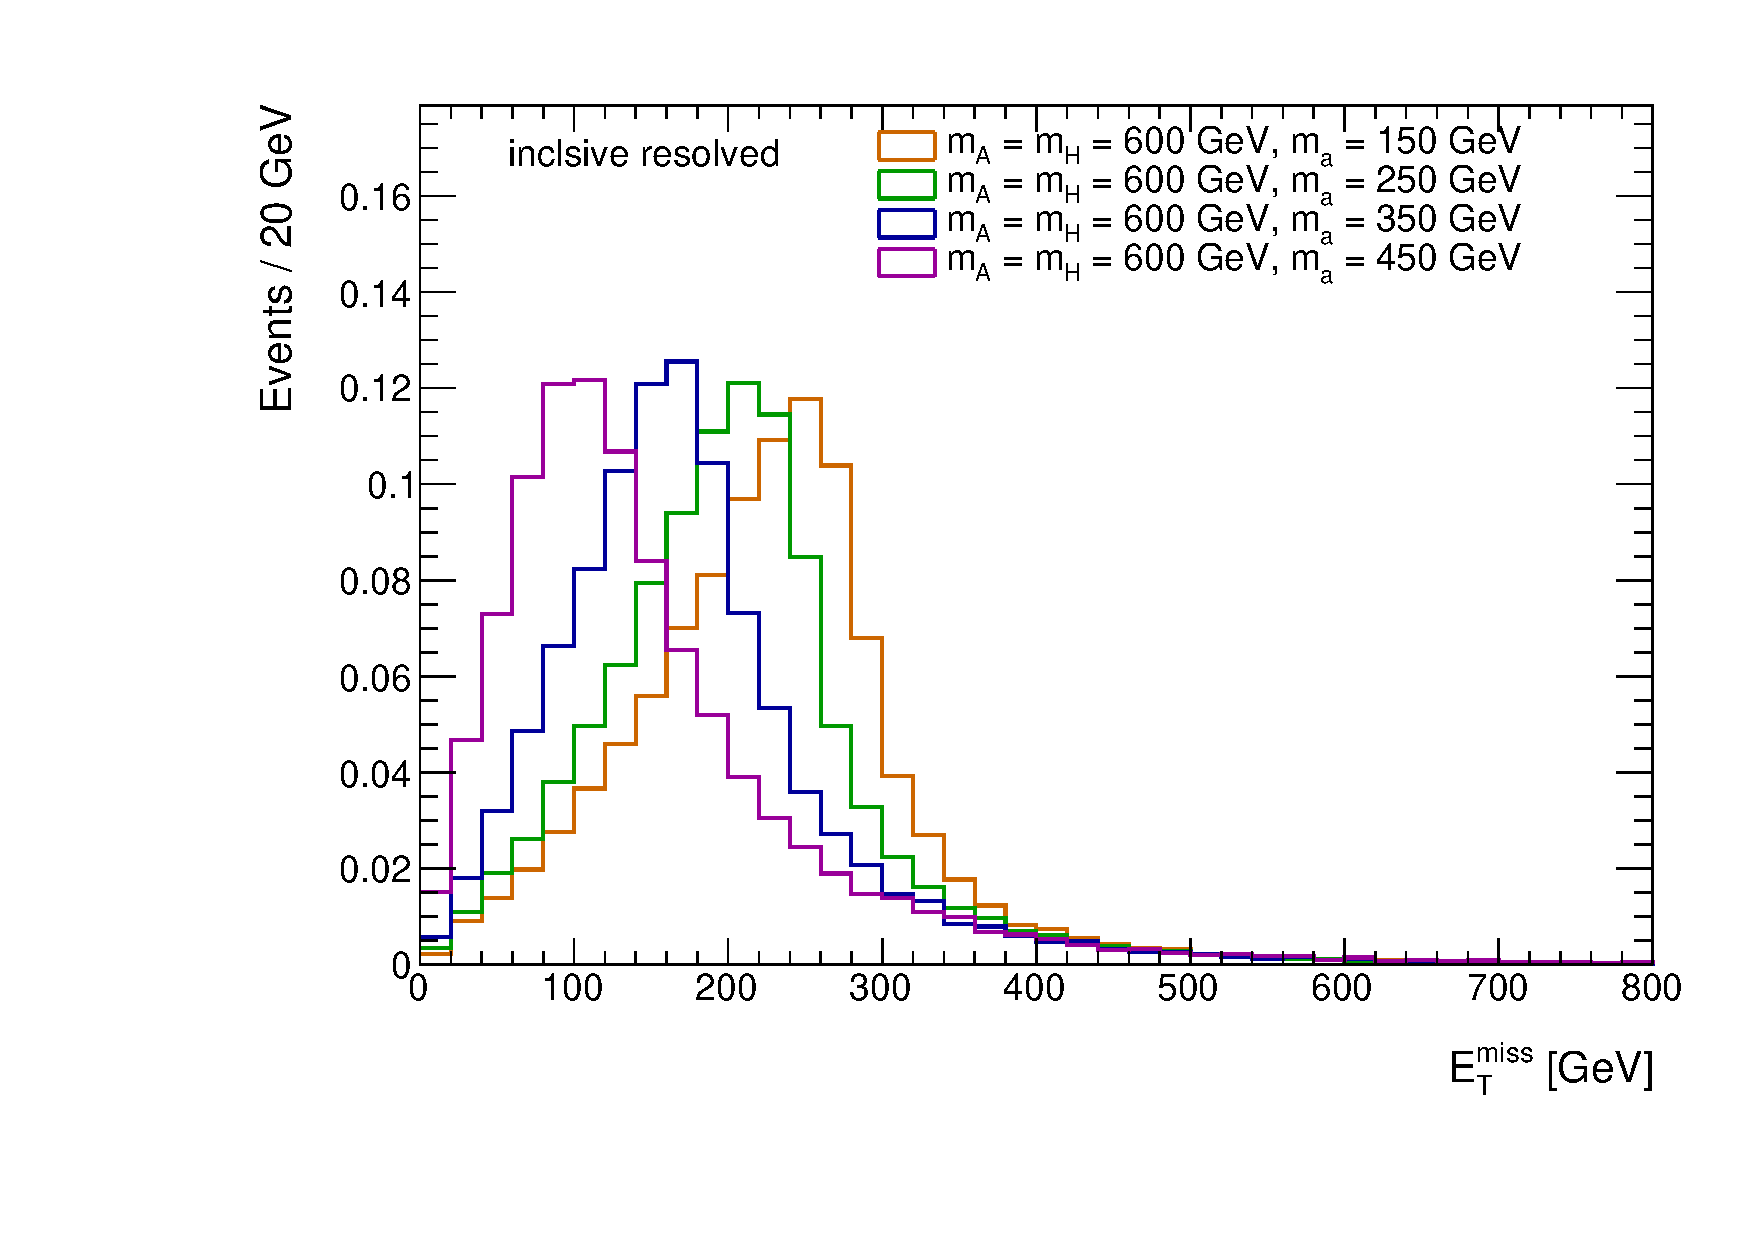
\includegraphics[width=0.45\textwidth]{texinputs/04_grid/figures/monoz/hadronic/mA600_incl_resl_MET_linear.pdf}
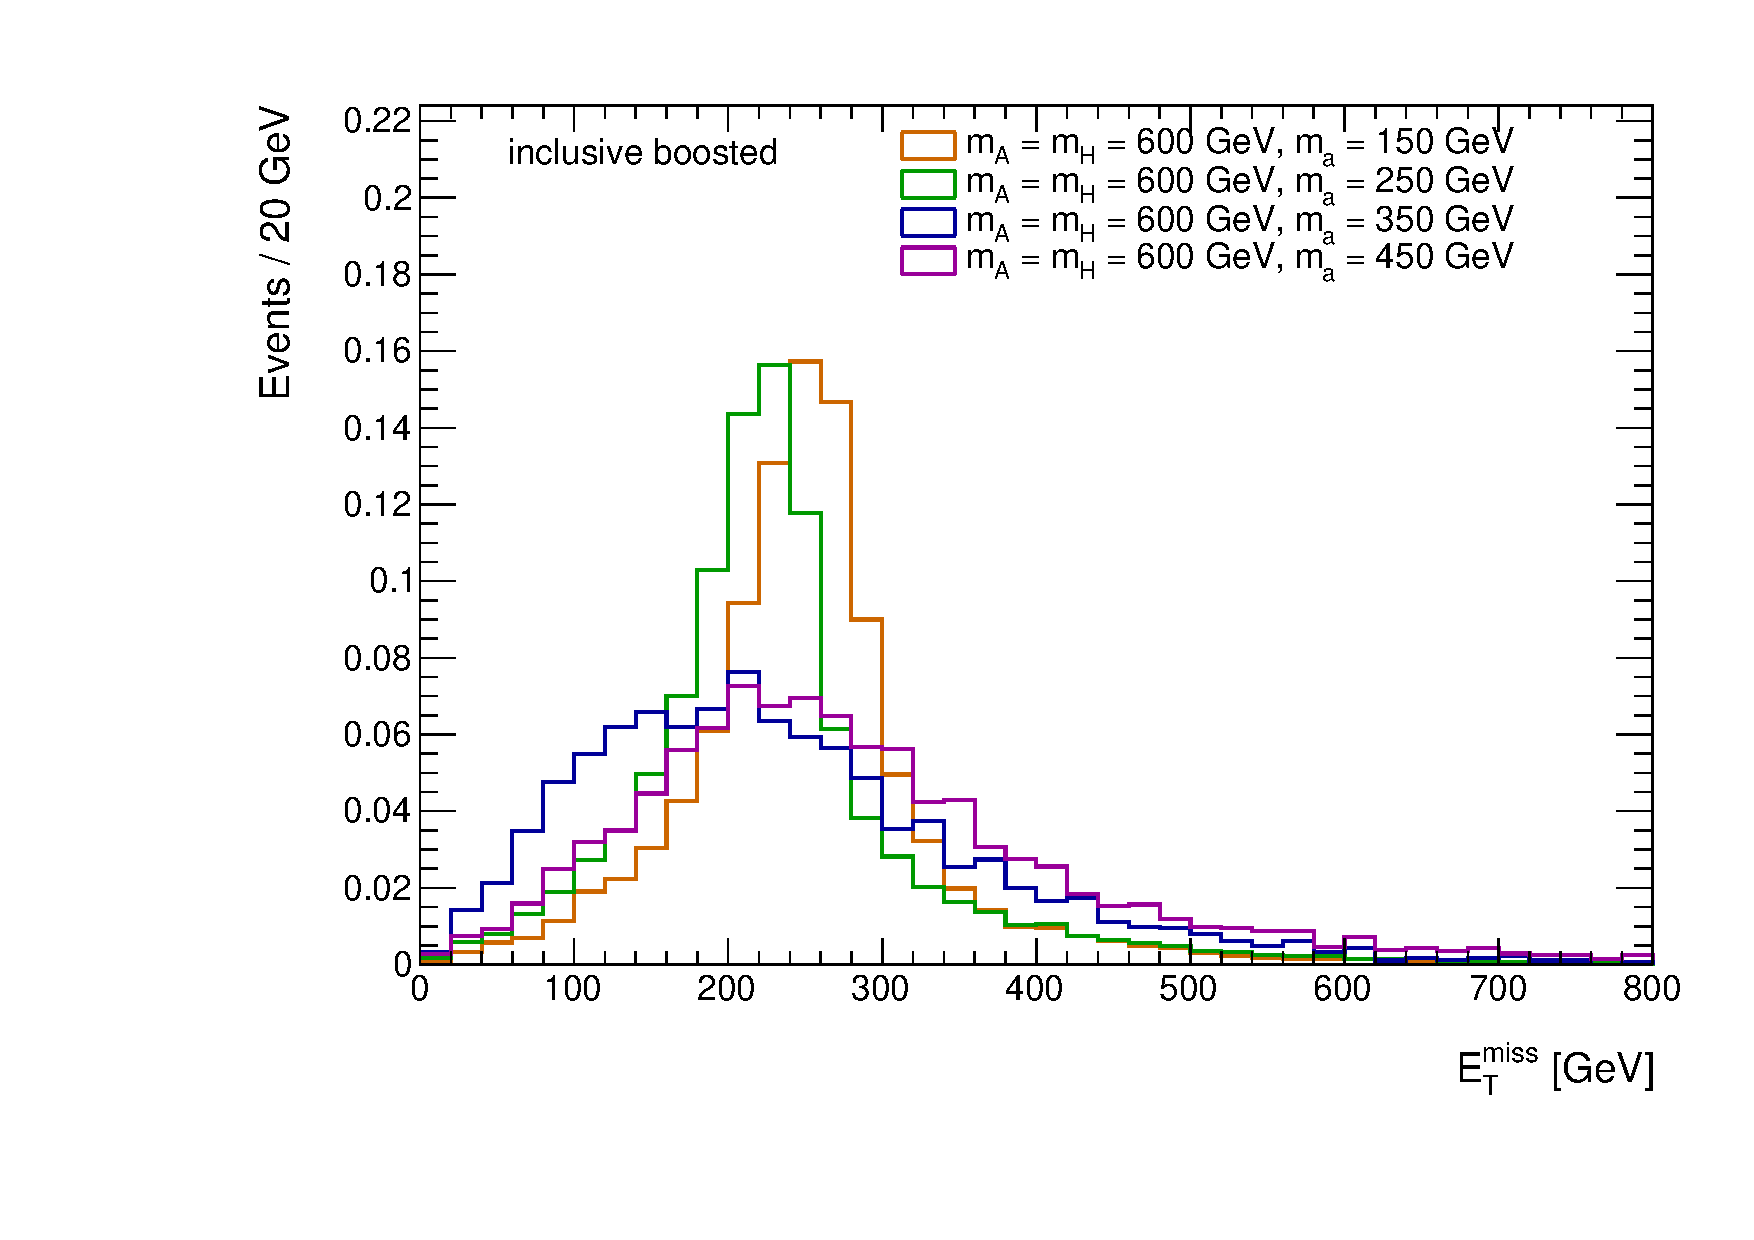
\includegraphics[width=0.45\textwidth]{texinputs/04_grid/figures/monoz/hadronic/mA600_incl_merged_MET_linear.pdf}
\caption{Dijet mass (top), $\Delta\Phi(jj, \MET)$ (middle) and $\MET$ (bottom) distributions 
after applying the inclusive selections in the resolved analysis are shown on the left side. Large-radius 
jet mass (top), $\Delta\Phi(J, \MET)$ (middle) and $\MET$ (bottom) distributions 
after applying the inclusive selections in the boosted analysis are shown on the right side. 
The signal masses are chosen to be \ma = 150, 250, 350 and 450~GeV with the fixed \mA = 600~GeV.}
\label{fig:monozhad_kin_inc_fixed_mA}
\end{figure}

Figure~\ref{fig:monozhad_kin_inc_fixed_ma} shows the kinematic distributions of mono-$Z$ events after applying 
the inclusive selections, separately for the resolved and boosted topologies. The \ma is fixed to 250~GeV and the \mA is
chosen to be 300, 600, 900 and 1200~GeV in the figure. When the \mA gets closer to \ma, the $Z$-boson
is less boosted, causing the large-radius jet mass to be more populated at mass below $\sim30$~GeV. 
When the $|\mA-\ma|$ becomes smaller than the $Z$-boson mass, the non-resonant production dominates as clearly
seen in the \MET spectrum for the resolved case.
Figure~\ref{fig:monozhad_kin_inc_fixed_mA} shows the same set of distributions when the \mA is fixed to 600~GeV 
and the \ma varies from 150 to 250, 350 and 450~GeV. 
The trend seen in Fig.~\ref{fig:monozhad_kin_inc_fixed_ma} is also visible here when the \ma gets closer to \mA.


\begin{figure}
\centering
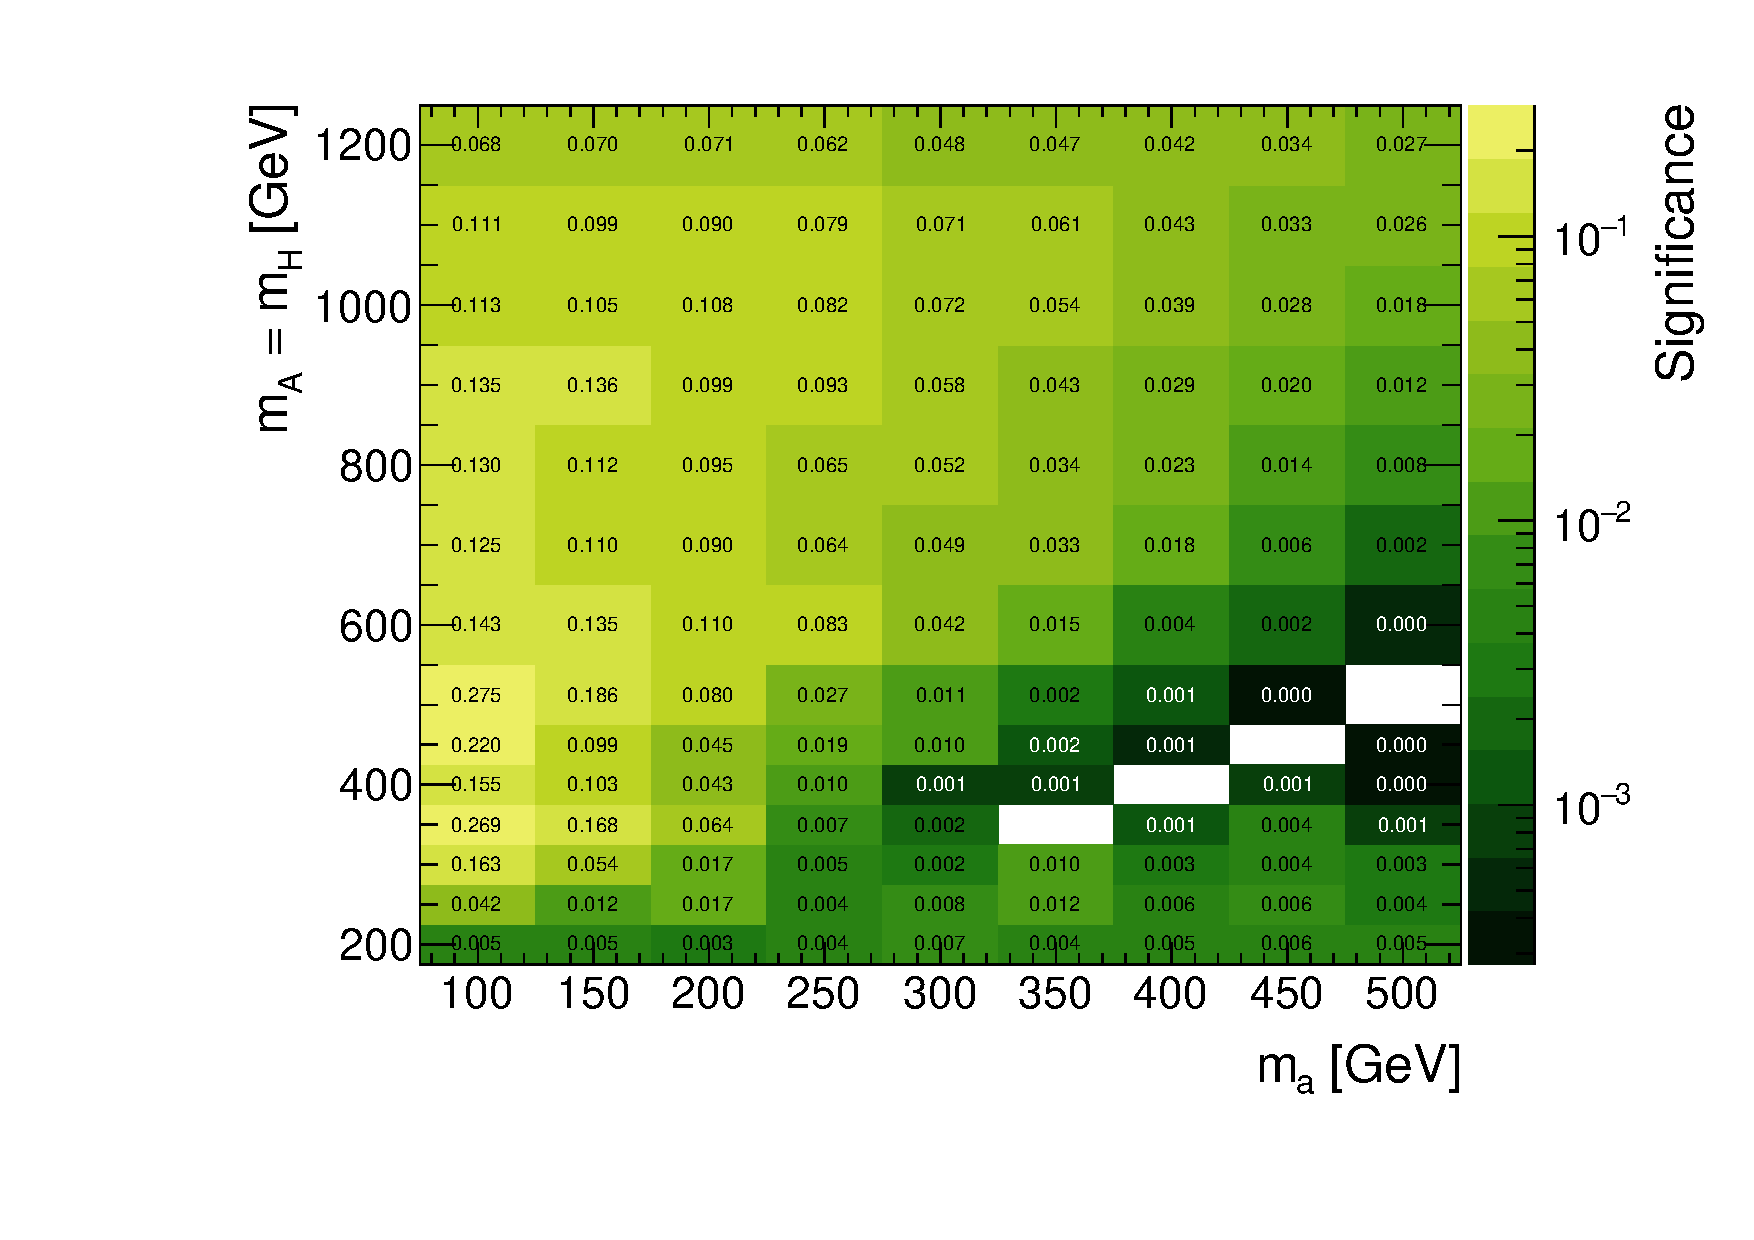
\includegraphics[width=0.45\textwidth]{texinputs/04_grid/figures/monoz/hadronic/grid_mA_ma_resl_bin100_sign_type3_bkg_uncert_0p10.pdf}
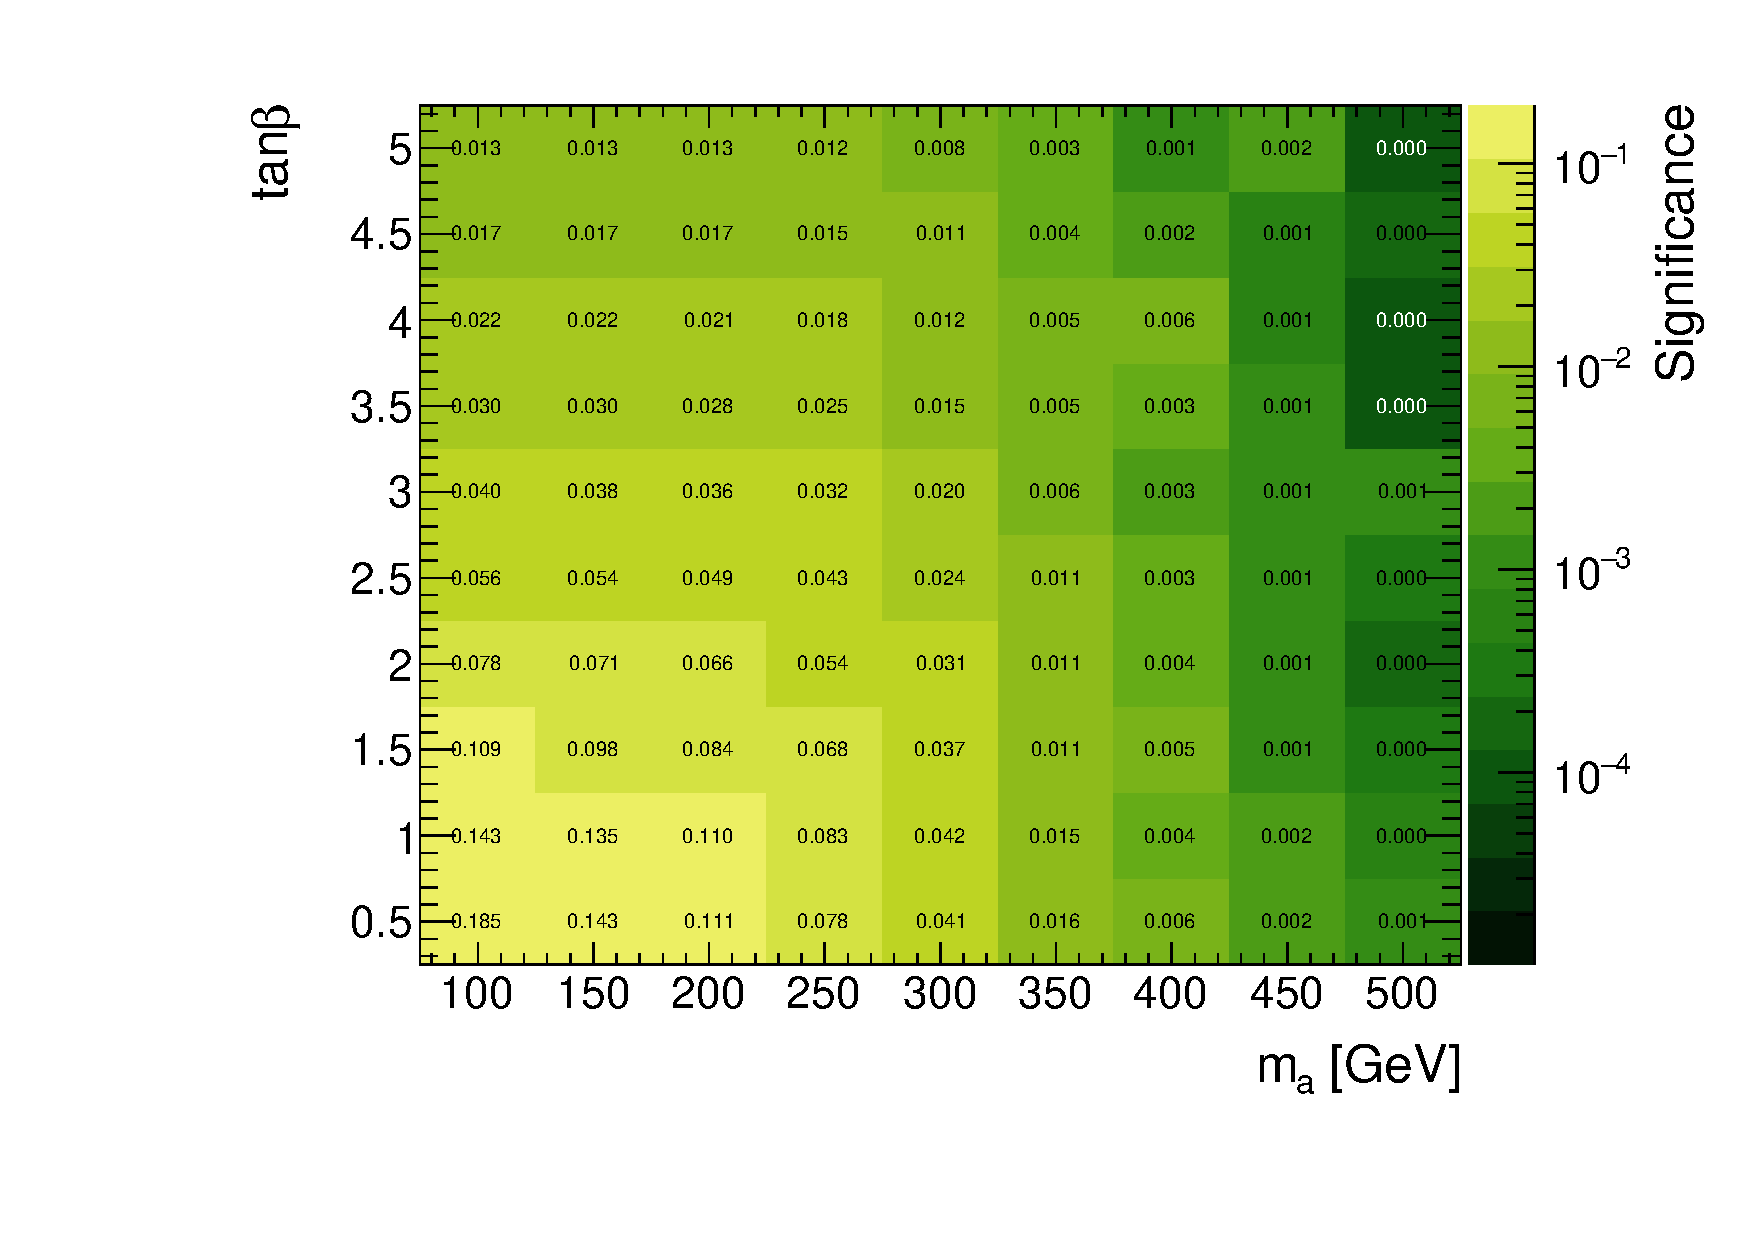
\includegraphics[width=0.45\textwidth]{texinputs/04_grid/figures/monoz/hadronic/grid_tanb_ma_resl_bin100_sign_type3_bkg_uncert_0p10.pdf}
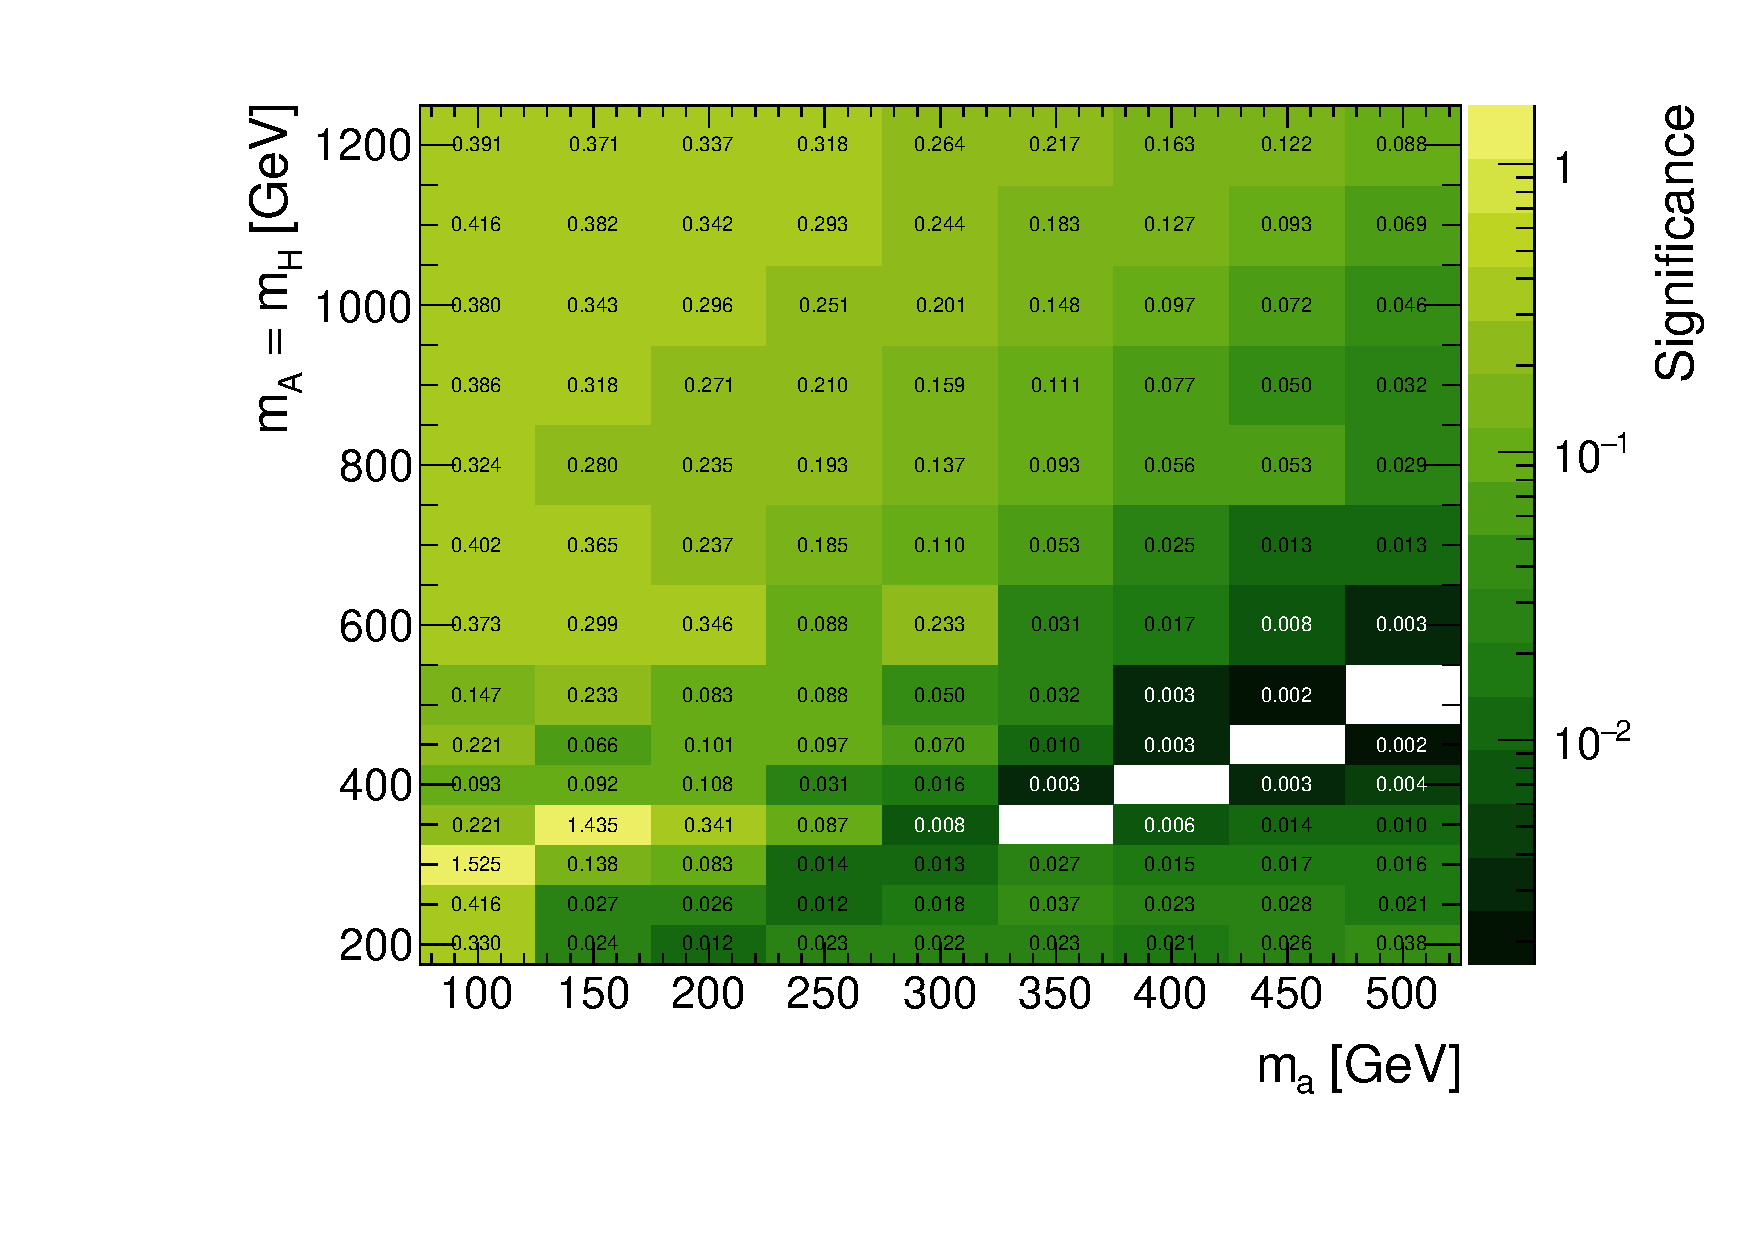
\includegraphics[width=0.45\textwidth]{texinputs/04_grid/figures/monoz/hadronic/grid_mA_ma_merged_bin100_sign_type3_bkg_uncert_0p10.pdf}
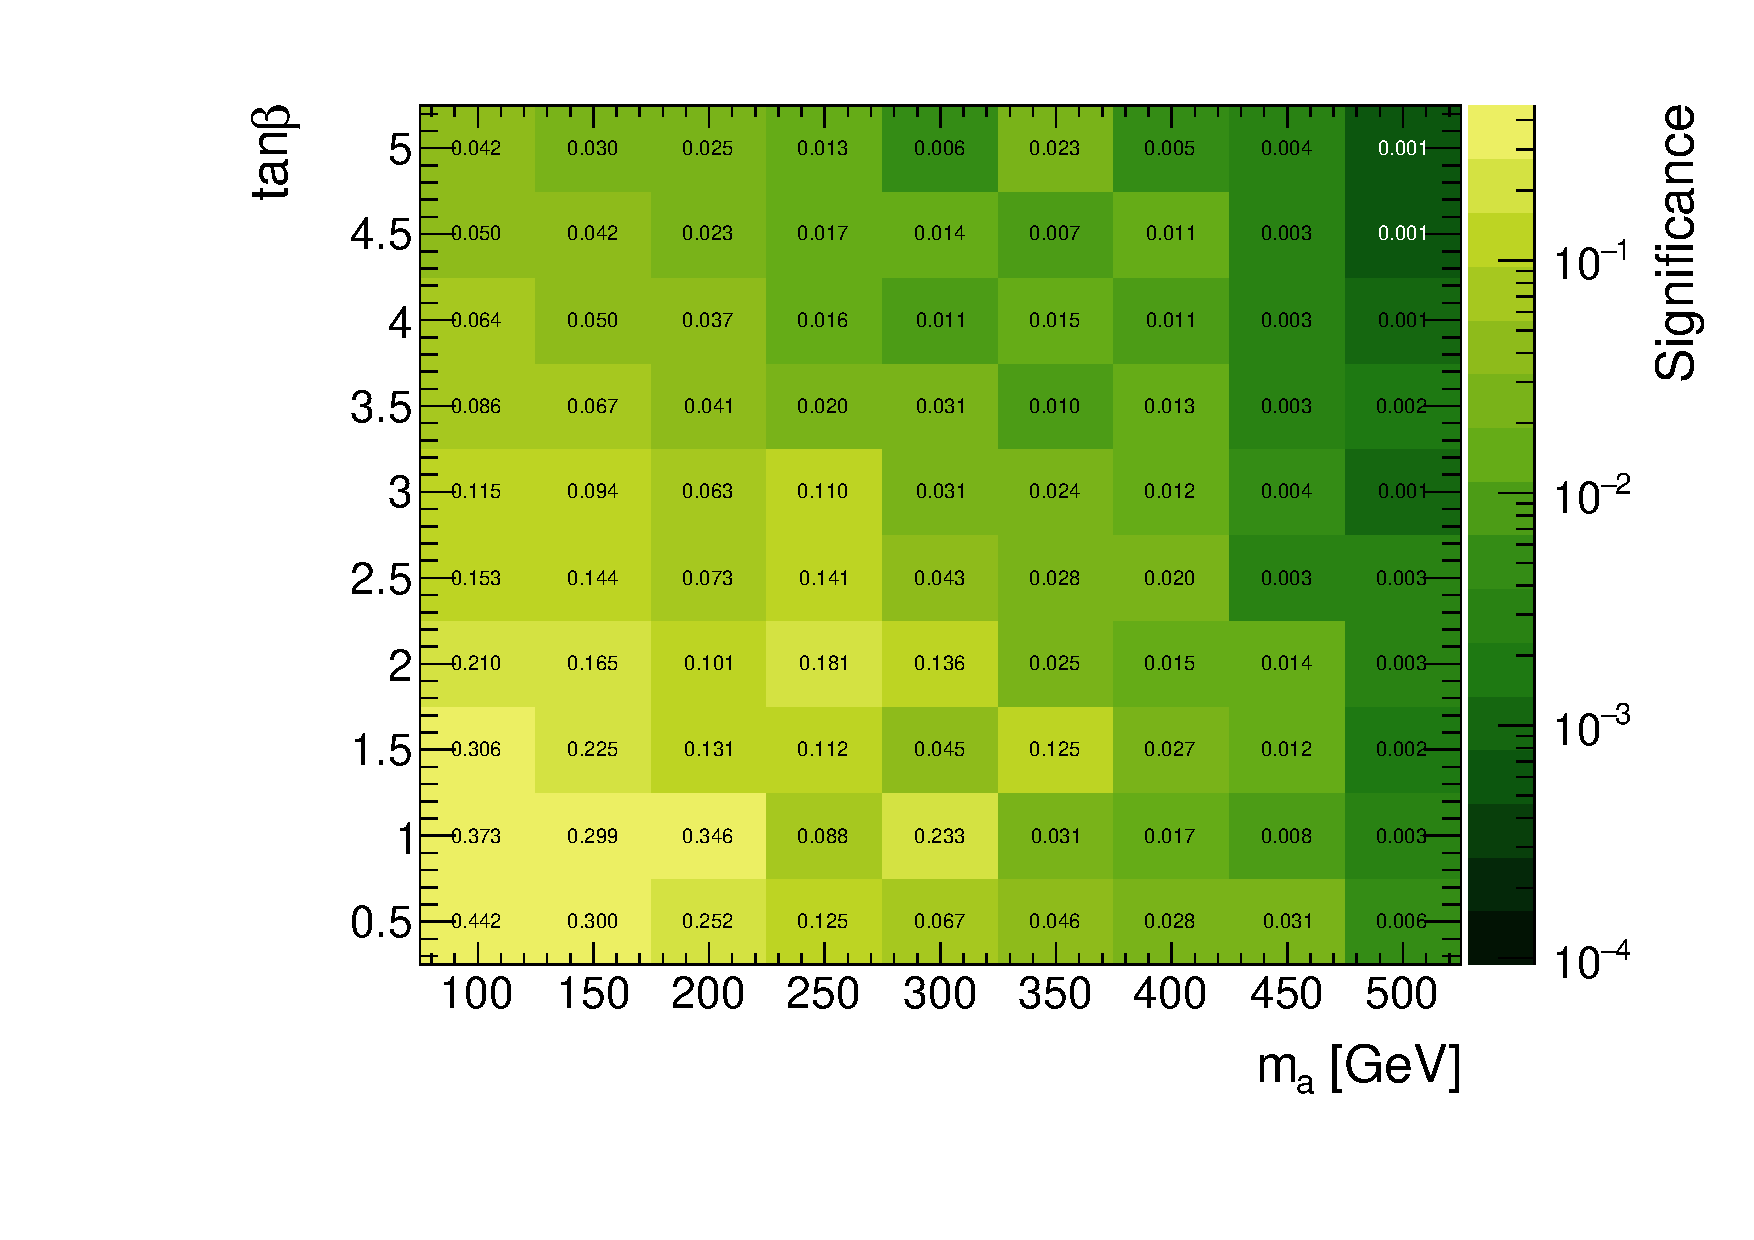
\includegraphics[width=0.45\textwidth]{texinputs/04_grid/figures/monoz/hadronic/grid_tanb_ma_merged_bin100_sign_type3_bkg_uncert_0p10.pdf}
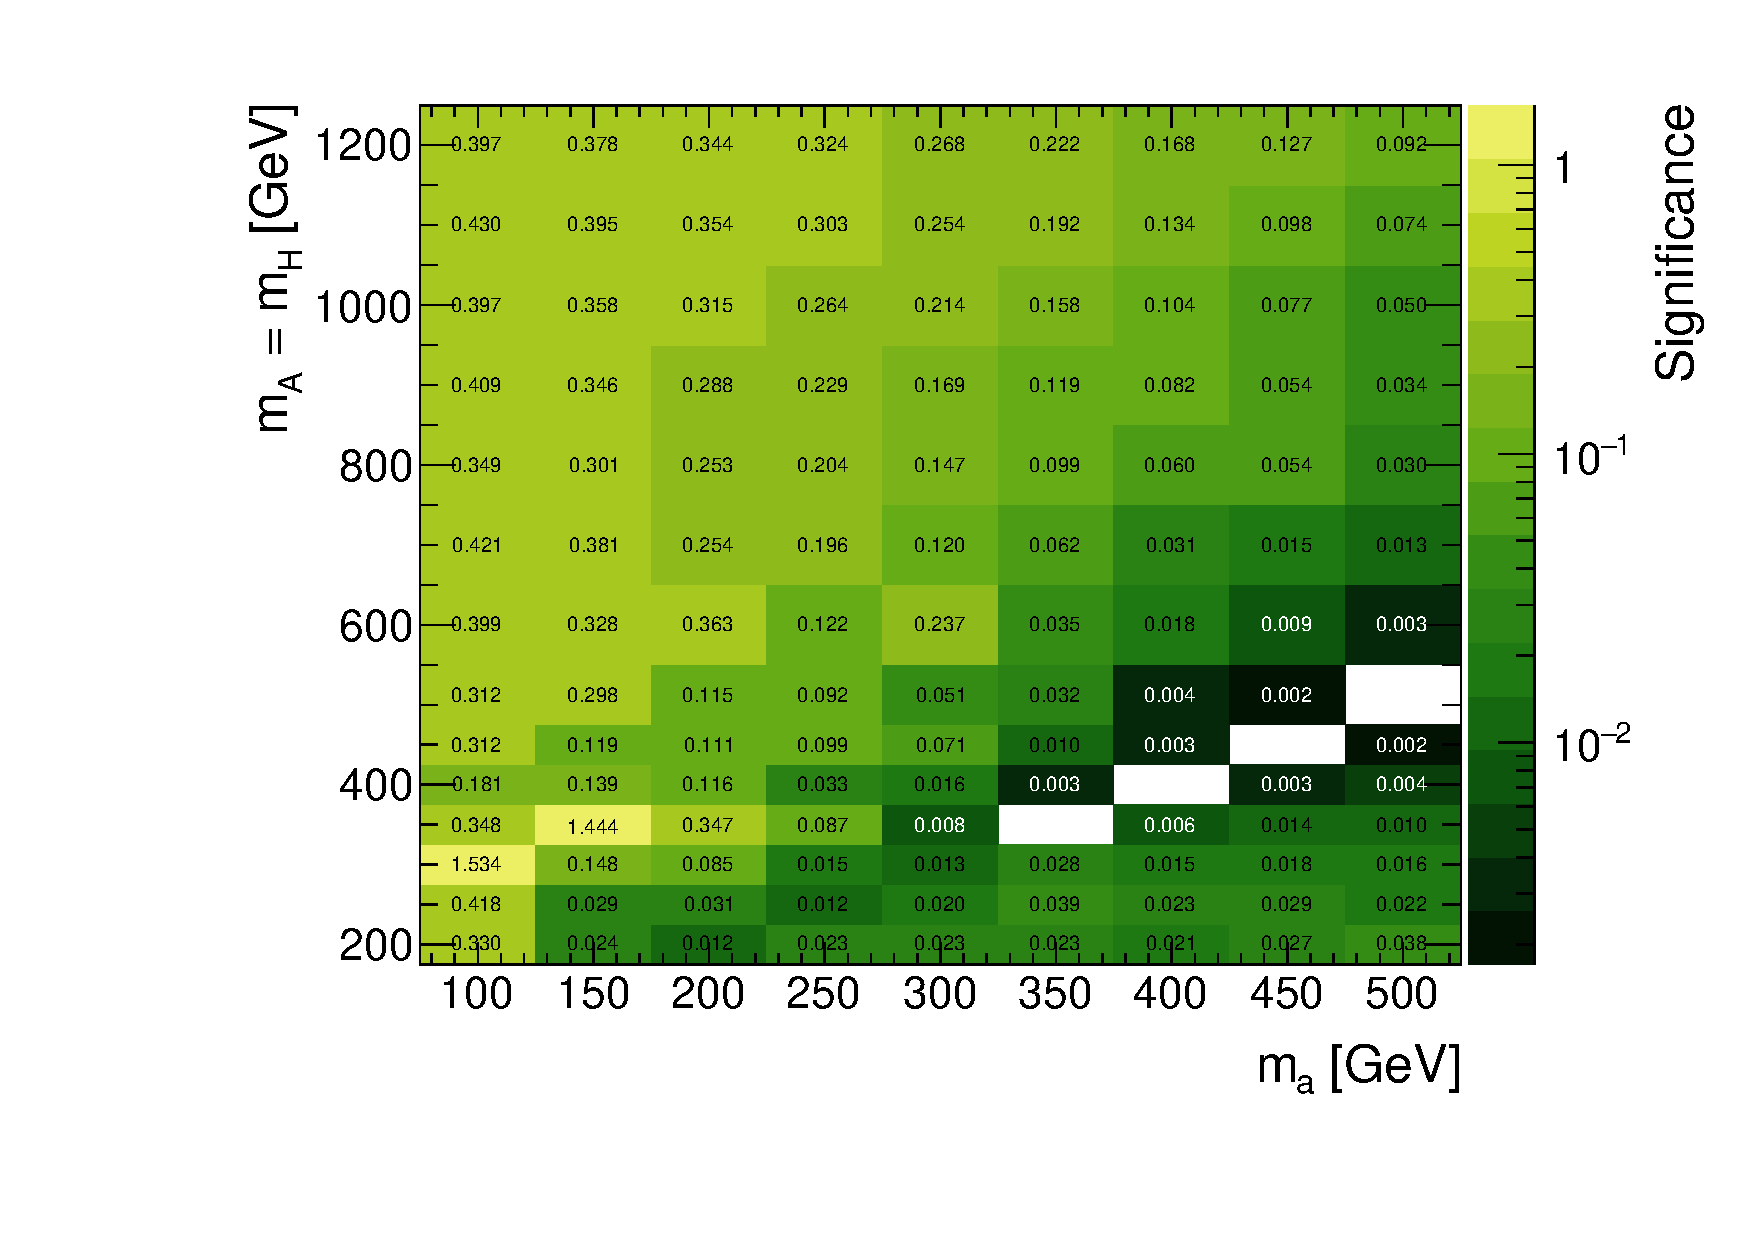
\includegraphics[width=0.45\textwidth]{texinputs/04_grid/figures/monoz/hadronic/grid_mA_ma_sum_bin100_sign_type3_bkg_uncert_0p10.pdf}
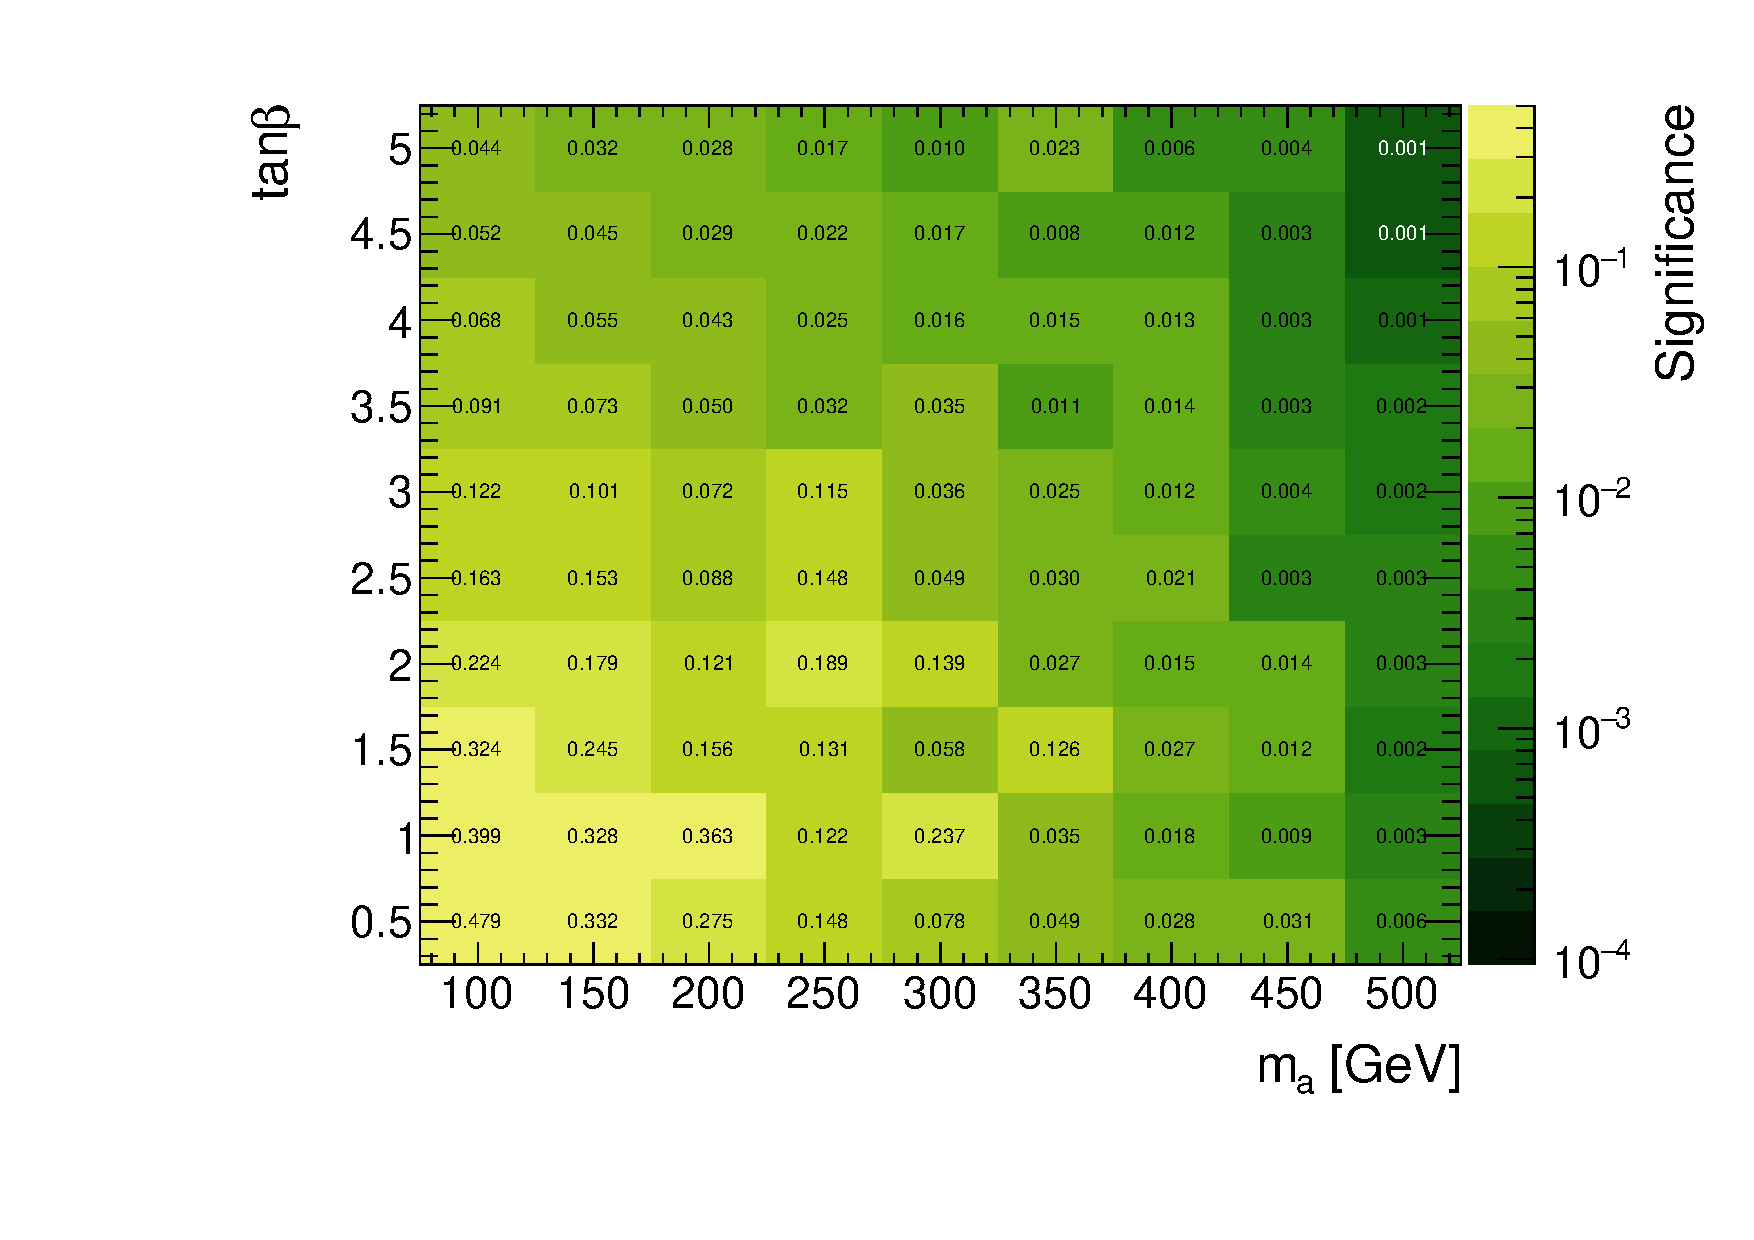
\includegraphics[width=0.45\textwidth]{texinputs/04_grid/figures/monoz/hadronic/grid_tanb_ma_sum_bin100_sign_type3_bkg_uncert_0p10.pdf}
\caption{Significance (as defined in the text) for the mono-$Z$ hadronic events 
$pp \rightarrow Z(\to q\bar{q})\chi\overline{\chi}$ in the \ma vs \mA (left) and \ma vs $\tan\beta$ (right) grids. 
Shown at the top, middle and bottom are the resolved only, boosted only and the combined resolved+boosted 
analysis, respectively.}
\label{fig:monozhad_significance_grid}
\end{figure}

The sensitivity of the resolved, boosted and the combined analysis selections to the mono-$Z$ hadronic signature 
is examined. The main background for this signature is $Z \to \nu\nu$ events in association with jets. 
The sample of $Z (\to \nu\nu)$+jets events is produced using Sherpa~2.2.1 and the matrix elements are calculated
up to 2 partons at next-to-leading order and up to 4 partons at leading order. The $Z (\to \nu\nu)$+jets events
are analyzed at particle level with the same criteria used for the signal. The number of $Z \to \nu\nu$ events 
after applying the cuts is increased by a factor 2 to account for the contribution from other backgrounds. 
This factor is chosen from the 
ATLAS dark matter search in the mono-$Z$ hadronic signature using 3.2~fb$^{-1}$ of 13~TeV data,
published in Ref.~\ref{EXOT-2015-08}. The sensitivity is defined in this study as 
%
\begin{equation}
\text{Significance} = \sqrt{\sum_{\text{bin}} Z_{\text{bin}}^2}
\label{eq:monozhad_sig}
\end{equation}
%
where the per-bin significance, $Z_{\text{bin}}$, is obtained, using asymptotic calculation of the 
Poisson likelihood ratio statistic, to be 
%
\begin{equation}
Z_{\text{bin}} = \left[ 2\left( (s+b)\ln \left[ \frac{(s+b)(b+\sigma_b^2)}{b^2+(s+b)\sigma_b^2} \right] - \frac{b^2}{\sigma_b^2} \ln \left[ 1+\frac{\sigma_b^2 s}{b(b+\sigma_b^2)} \right] \right) \right]^{1/2} 
\end{equation}
%
with the assumption of 10\% background uncertainty in each \MET bin. 
The sum in Eq.(\ref{eq:monozhad_sig}) is taken over all \MET bins after applying the final selections.
The results are shown in Fig.~\ref{fig:monozhad_significance_grid} for the resolved only, booted only and 
the combined resolved+boosted analysis selections, corresponding to the integrated luminosity of 40~fb$^{-1}$
at $\sqrt{s} = 13$~TeV. The significance depends strongly on the assumption of background uncertainty 
since a large number of background events remain in this simple analysis with a minimum set of selection criteria.
More realistic analysis performed in LHC experiments is expected to improve the sensitivity.

